\documentclass[../../main]{subfiles}
\pagestyle{fancy}

\begin{document}

\chapter{Virtual large cardinals}
\thispagestyle{fancy}

In this chapter we investigate the properties of virtual versions of well-known large cardinals, including measurables, strongs, supercompacts, woodins and vop\v enkas. This entails firstly analysing the relationships between them, and secondly looking at more general properties in terms of their behaviour in canonical inner models as well as their indestructibility. This virtual perspective also allows us to analyse virtualised versions of large cardinals that are otherwise inconsistent with $\zfc$, such as the berkeley cardinals.


\section{Strongs \& supercompacts}

We start out with measurables, strongs and supercompacts. Their (non-virtual) definitions can be found in Appendix \ref{apx.large-cardinals}.

\defi[][defi.strongsc]{
  Let $\theta$ be a regular uncountable cardinal. Then a cardinal $\kappa<\theta$ is...
  \begin{itemize}
    \item \textbf{faintly $\theta$-measurable} if, in a forcing extension, there is a transitive class $\N$ and an elementary embedding $\pi\colon H_\theta^V\to\N$ with $\crit\pi=\kappa$;
    \item \textbf{faintly $\theta$-strong} if it's faintly $\theta$-measurable, $H_\theta^V\subset\N$ and $\pi(\kappa)>\theta$;
    \item \textbf{faintly $\theta$-supercompact} if it's faintly $\theta$-measurable, ${^{<\theta}\N}\subset\N$ and $\pi(\kappa)>\theta$.
  \end{itemize}

  We further replace ``faintly'' by \textbf{virtually} when $\N\subset V$, we attach a \textbf{``pre''} if we don't assume that $\pi(\kappa)>\theta$, and we will leave out $\theta$ when it holds for all regular $\theta>\kappa$.
}

As a quick example of this terminology, a \textit{faintly prestrong cardinal} is a cardinal $\kappa$ such that for all regular $\theta>\kappa$, $\kappa$ is faintly $\theta$-measurable with $H_\theta^V\subset\N$.

\qquad We note that even small cardinals can be faintly measurable: we may for instance have a precipitous ideal on $\omega_1$; see \cite[Theorem 22.33]{Jech}. The ``virtually'' adverb implies that the cardinals are in fact large cardinals in the usual sense, as Proposition \ref{prop.virtit} below shows.

\prop[Virtualised folklore][prop.virtit]{
  For any regular uncountable cardinal $\theta$, every virtually $\theta$-measurable cardinal is 1-iterable.
}
\proof{
  Let $\kappa$ be virtually $\theta$-measurable, witnessed by a forcing $\mathbb P$, a transitive $\N\subset V$ and an elementary $\pi\colon H_\theta^V\to\N$ with $\pi\in V^{\mathbb P}$. If $\kappa$ isn't a strong limit then we have a surjection $\pi(f)\colon\p(\alpha)\to\pi(\kappa)$ with $\ran\pi(f)=\ran f\subset\kappa$ for some $\alpha<\kappa$, $\contr$. Note that we used $\N\subset V$ to ensure that $\p(\alpha)^V=\p(\alpha)^{\N}$. The same argument shows that $\kappa$ is regular. By restricting the generic embedding and using that $\p(\kappa)^V = \p(\kappa)^N$ as $\N\subset V$ and $\p(\kappa)^V\subset\N$, we get that $\kappa$ is 1-iterable.
}

Along with the above definition of faintly supercompactness we can also virtualise Magidor's characterisation of supercompact cardinals\footnote{See Appendix \ref{apx.large-cardinals} for the non-virtual version of this characterisation.}, which was one of the original characterisations of the remarkable cardinals in \cite{Schindler}.

\defi{
  Let $\theta$ be a regular uncountable cardinal. Then a cardinal $\kappa<\theta$ is \textbf{virtually $\theta$-Magidor-supercompact} if there are $\bar\kappa<\bar\theta<\kappa$ and a generic elementary $\pi\colon H_{\bar\theta}^V\to H_\theta^V$ such that $\crit\pi=\bar\kappa$ and $\pi(\bar\kappa)=\kappa$.
}

In the virtual world these two versions of supercompacts remain equivalent, but they also turn out to be equivalent to the virtually strongs:

\theo[Gitman-Schindler][theo.rem]{
  For an uncountable cardinal $\kappa$, the following are equivalent.\footnote{A cardinal satisfying any/all of these conditions is usually called \textbf{remarkable}.}
  \begin{enumerate}
    \item $\kappa$ is virtually strong;
    \item $\kappa$ is virtually supercompact;
    \item $\kappa$ is virtually Magidor-supercompact.
  \end{enumerate}
}
\proof{
$(ii)\Rightarrow(i)$ is simply by definition.

\qquad $(i)\Rightarrow (iii)$: Fix $\theta>\kappa$. By $(i)$ there exists a generic elementary embedding $\pi\colon H_{(2^{<\theta})^+}^V\to\M$ with\footnote{The domain of $\pi$ is $H_{(2^{<\theta})^+}^V$ to ensure that $H_\theta^V\in\dom\pi$.} $\crit\pi=\kappa$, $\pi(\kappa)>\theta$, $H_{(2^{<\theta})^+}^V\subset\M$ and $\M\subset V$. Since $H_\theta^V, H_{\pi(\theta)}^{\M}\in\M$, Countable Embedding Absoluteness \ref{lemm.ctblabs} implies that $\M$ has a generic elementary embedding $\pi^*:H_\theta^V\to H_{\pi(\theta)}^{\M}$ with $\crit\pi^*=\kappa$ and $\pi^*(\kappa)=\pi(\kappa)>\theta$. Since $H_\theta^V=H_\theta^{\M}$ as $\M\subset V$ and $H_\theta^V\subset\M$, elementarity of $\pi$ now implies that $H_{(2^{<\theta})^+}^V$ has ordinals $\bar\kappa<\bar\theta<\kappa$ and a generic elementary $\sigma\colon H_{\bar\theta}^V\to H_\theta^V$ with $\crit\sigma=\bar\kappa$ and $\sigma(\bar\kappa)=\kappa$. This shows $(iii)$.

  \qquad $(iii)\Rightarrow (ii)$: Fix $\theta>\kappa$ and $\delta:=(2^{<\theta})^+$. By $(iii)$ there exist ordinals $\bar\kappa<\bar\delta<\kappa$ and a generic elementary embedding $\pi\colon H_{\bar\delta}^V\to H_\delta^V$ with $\crit\pi=\bar\kappa$ and $\pi(\bar\kappa)=\kappa$. We will argue that $\bar\kappa$ is virtually $\bar\theta$-supercompact in $H_{\bar\delta}^V$, so that by elementarity $\kappa$ is virtually $\theta$-supercompact in $H_\delta^V$ and hence also in $V$ by the choice of $\delta$. Consider the restriction
  \eq{
    \sigma:=\pi\restr H_{\bar\theta}^V\colon H_{\bar\theta}^V\to H_\theta^V.
  }

  Note that $H_\theta^V$ is closed under ${<}\bar\theta$-sequences (and more) in $V$. Now define
  \eq{
    X := \bar\theta{+}1 \cup \{x\in H_\theta^V\mid\exists y\in H_{\bar\theta}^V\exists p\in\col(\omega, H_{\bar\theta}^V)\colon p\forces\dot\sigma(\check y)=\check x\}\in V.
  }

  Note that $\abs X = \abs{H_{\bar\theta}^V} = 2^{<\bar\theta}$ and that $\ran\sigma\subset X$. Now let $\overline\M\prec H_\theta^V$ be such that $X\subset\overline\M$ and $\overline\M$ is closed under ${<}\bar\theta$-sequences. Note that we can find such an $\overline\M$ of size $(2^{<\bar\theta})^{<\bar\theta} = 2^{<\bar\theta}$. Let $\M$ be the transitive collapse of $\overline\M$, so that $\M$ is still closed under ${<}\bar\theta$-sequences and we still have that $\abs\M = 2^{<\bar\theta}<\bar\delta$, making $\M\in H_{\bar\delta}^V$.

  \qquad Countable Embedding Absoluteness \ref{lemm.ctblabs} then implies that $H_{\bar\delta}^V$ has a generic elementary embedding $\sigma^*\colon H_{\bar\theta}^V\to\M$ with $\crit\sigma^*=\bar\kappa$, showing that $\bar\kappa$ is virtually $\bar\theta$-supercompact in $H_{\bar\delta}^V$, which is what we wanted to show.
}

\rema{
  The above proof in fact shows something stronger: if $\kappa$ is virtually $(2^{<\theta})^+$-strong then it is virtually $\theta$-supercompact, and if it's virtually $(2^{<\theta})^+$-Magidor-supercompact then it's virtually $\theta$-supercompact. It's open whether they are equivalent level-by-level (see Question \ref{ques.remarkableequiv}).
}

A key difference between the normal large cardinals and the virtual kind is that we don't have a virtual version of the Kunen inconsistency\footnote{See Appendix \ref{apx.large-cardinals} for the Kunen inconsistency.}: it's perfectly valid to have a generic elementary embedding $H_\theta^V\to H_\theta^V$ with $\theta$ much larger than the critical point.

\prop[Folklore]{
  If $0^\sharp$ exists then there are inaccessible cardinals $\kappa<\theta$ such that, in a generic extension of $L$, there is an elementary embedding $\pi\colon L_\theta\to L_\theta$. In other words, $\pi$ witnesses a strong failure of the virtualised Kunen inconsistency.
}
\proof{
  From $0^\sharp$ we get an elementary embedding $j\colon L\to L$. Let $C\subset\on$ be the proper class club of limit points of $j$ above $\crit j$, which then contains an inaccessible cardinal $\theta$ as there are stationarily many such. Restrict $j$ to $\pi:=j\restr L_\theta\to\N$ and note that $\N=L_\theta$ by condensation and because $\theta$ is a limit point of $j$. Let $\kappa:=\crit\pi$. Now an application of Countable Embedding Absoluteness \ref{lemm.ctblabs} shows that a generic extension of $L$ contains an elementary embedding $\tilde\pi: L_\theta\to L_\theta$ with $\crit\tilde\pi = \kappa$.
}

This becomes important when dealing with the ``pre''-versions of the large cardinals. We next move to a virtualisation of the $\alpha$-superstrong cardinals.

\defi[N.]{
  Let $\theta$ be a regular uncountable cardinal and and $\alpha$ an ordinal. Then a cardinal $\kappa<\theta$ is \textbf{faintly $(\theta,\alpha)$-superstrong} if it's faintly $\theta$-measurable, $H_\theta^V\subset\N$ and $\pi^\alpha(\kappa)\leq\theta$\footnote{Here we set $\pi^\alpha(\kappa) := \sup_{\xi<\alpha}\pi^\xi(\kappa)$ when $\alpha$ is a limit ordinal.}. We replace ``faintly'' by \textbf{virtually} when $\N\subset V$, we say that $\kappa$ is \textbf{faintly $\alpha$-superstrong} if it's faintly $(\theta,\alpha)$-superstrong for \textit{some} $\theta$, and lastly $\kappa$ is simply \textbf{faintly superstrong} if it is faintly 1-superstrong.\footnote{Note that the conventions stated here are different from the ones in Definition \ref{defi.strongsc}.}
}

As in the non-virtual case, the virtually superstrongs supercede the virtually strongs in consistency strength. Note that this then also implies that the superstrongs are stronger than the virtually supercompacts, which is \textit{not} the case outside the virtual world.

\prop[N.][prop.superstrong]{
  If $\kappa$ is faintly superstrong then $H_\kappa$ has a proper class of virtually strong cardinals.
}
\proof{
  Fix a regular $\theta>\kappa$ and a generic embedding $\pi\colon H_\theta^V\to\N$ with $\crit\pi=\kappa$, $H_\theta^V\subset\N$ and $\pi(\kappa)<\theta$. Then $\pi(\kappa)$ is a $V$-cardinal, so that $H_{\pi(\kappa)}^V$ thinks that $\kappa$ is virtually strong. This implies that $H_\kappa^V$ thinks there is a proper class of virtually strong cardinals, using that $H_\kappa^V\prec H_{\pi(\kappa)}^V$.
}

The following theorem then shows that the only thing stopping prestrongness from being equivalent to strongness is the existence of ``Kunen inconsistencies''. 

\theo[N.][theo.virtchar]{
  Let $\theta$ be an uncountable cardinal. Then a cardinal $\kappa<\theta$ is virtually $\theta$-prestrong iff either
  \begin{enumerate}
    \item $\kappa$ is virtually $\theta$-strong; or
    \item $\kappa$ is virtually $(\theta,\omega)$-superstrong.
  \end{enumerate}
}
\proof{
  $(\Leftarrow)$ is trivial, so we show $(\Rightarrow)$. Let $\kappa$ be virtually $\theta$-prestrong. Assume $(i)$ fails, meaning that there's a generic extension $V^{\mathbb P}$ and an elementary embedding $\pi\in V^{\mathbb P}$ such that $\pi\colon H_\theta^V\to\N$ for some transitive $\N$ with $H_\theta^V\subset\N$, $\N\subset V$, $\crit\pi=\kappa$ and $\pi(\kappa)\leq\theta$. Assume $\pi^n(\kappa)$ is defined for all $n<\omega$ and define $\lambda := \sup_{n<\omega}\pi^n(\kappa)$. If $\lambda\leq\theta$ then $\kappa$ is virtually $(\theta, \omega)$-superstrong by definition, so assume that there's some least $n<\omega$ such that $\pi^{n+1}(\kappa)>\theta$.

  \qquad This means that $\kappa$ is virtually $\nu$-strong for every regular $\nu\in(\kappa,\pi^n(\kappa))$, which is a $\Delta_0$-statement in $\{H_{\nu^+}^V\}$ and hence downwards absolute to $H_{\pi^n(\kappa)}^V$. This means that $\kappa$ is virtually strong in $H_{\pi^n(\kappa)}^V$ and also that $\pi^n(\kappa)$ is virtually strong in $H_{\pi^{n+1}(\kappa)}^{\N}$ by elementarity, and so in particular virtually $\theta$-strong in $\N$. This means that there's some generic elementary embedding
  \eq{
    \sigma\colon H_\theta^{\N}\to\M
  }

  with $H_\theta^{\N}\subset\M$, $\M\subset\N$, $\crit\sigma=\pi^n(\kappa)$ and $\sigma(\pi^n(\kappa))>\theta$. We can now restrict $\sigma$ to its critical point $\pi^n(\kappa)$ to get that
  \eq{
    H_{\pi^n(\kappa)}^V = H_{\pi^n(\kappa)}^{\N} \prec H_{\sigma(\pi^n(\kappa))}^{\M},
  }

  using that $H_\theta^V = H_\theta^{\N}$ holds as $\pi$ is a virtual embedding. Since $\kappa$ is virtually strong in $H_{\pi^n(\kappa)}^V$ this means that $\kappa$ is also virtually strong in $H_{\sigma(\pi^n(\kappa))}^{\M}$. In particular, $\kappa$ is virtually $\theta$-strong in $\M$, and as $H_\theta^{\M} = H_\theta^{\N} = H_\theta^V$, this means that $\kappa$ is virtually $\theta$-strong in $V$, contradicting $(i)$.
}

We then get the following consistency result.

\coro[N.]{
  For any uncountable regular $\theta$, the existence of a virtually $\theta$-strong cardinal is equiconsistent with the existence of a faintly $\theta$-measurable cardinal.
}
\proof{
  The above Proposition \ref{prop.superstrong} and Theorem \ref{theo.virtchar} show that virtually $\theta$-prestrongs are equiconsistent with virtually $\theta$-strongs. Now note that Countable Embedding Absoluteness \ref{lemm.ctblabs} and condensation in $L$ imply that every faintly $\theta$-measurable cardinal is virtually $\theta$-prestrong in $L$.
}

Recall that a cardinal $\kappa$ is \textbf{virtually rank-into-rank} if there exists a cardinal $\theta>\kappa$ and a generic elementary embedding $\pi\colon H_\theta^V\to H_\theta^V$ with $\crit\pi=\kappa$. We firstly note that the virtually $\omega$-superstrongs coincide with the virtually rank-into-ranks.

\prop[N.][prop.superstrong-rank-into-rank]{
  A regular uncountable cardinal $\kappa$ is virtually $\omega$-superstrong iff it is virtually rank-into-rank.
}
\proof{
  If $\kappa$ is virtually $\omega$-superstrong, witnessed by a generic embedding $\pi\colon H_\theta^V\to\N$, then $\lambda:=\sup_{n<\omega}\pi^n(\kappa)$ is well-defined. By restricting $\pi$ to $\pi\restr H_\lambda^V\colon H_\lambda^V\to H_\lambda^V$ we get a witness to $\kappa$ being virtually $\lambda$-rank-into-rank.

  \qquad Conversely, if $\kappa$ is $\theta$-rank-into-rank, witnessed by a generic embedding $\pi\colon H_\theta^V\to H_\theta^V$, then one readily checks that $\pi$ also witnesses that $\kappa$ is virtually $\omega$-superstrong.
}



%%%%%%%%%%%%%%%%%%%%% SUPERSTRONG AND HUGE %%%%%%%%%%%%%%%%%%%%%%
\begin{comment}
\defi{
  \label{defi.strongsc}
  A cardinal $\kappa$ is...
  \begin{itemize}
    \item \textbf{faintly $\alpha$-superstrong} if it's faintly $\theta$-prestrong for some regular $\theta\geq\pi^\alpha(\kappa)$;
    \item \textbf{faintly $\alpha$-huge} if it's faintly $\theta$-presupercompact for some regular $\theta\geq\pi^\alpha(\kappa)$;
  \end{itemize}

  We replace ``faintly'' by \textbf{virtually} when $\N\subset V$, and when we don't specify any $\theta$ then it holds for \textbf{some} regular $\theta>\kappa$. When $\alpha=1$ we will usually leave it out.\footnote{So $\kappa$ is a faintly superstrong cardinal if there's a regular $\theta>\kappa$ and an elementary $\pi\colon H_\theta^V\to\N$ with $\crit\pi=\kappa$ and $H_{\pi(\kappa)}^V\subset\N$.}
}

With this terminology, by definition we have that every faintly $\theta$-prestrong cardinal is either faintly $\theta$-strong or faintly $\theta$-superstrong.

If we say that a cardinal $\kappa$ is \textit{virtually $n$-*huge} if it is virtually $n$-huge and the target model of the elementary embedding is of the form $H_\theta^V$ for some cardinal $\theta$, then Theorem 4.14 in \cite{GitmanSchindler} says the following.\footnote{In that paper they're working with $V_\alpha$'s instead of $H_\theta$'s, but the same proof goes through.}

\theo[Gitman-Schindler]{
  If $\kappa$ is $(n{+}2)$-iterable then
  \eq{
    H_\kappa^V\models\godel{\text{there is a proper class of virtually $n$-*huge cardinals}}.\tag*{$\dashv$}
  }
}

Note that every virtually $n$-*huge cardinal is a limit of virtually $n$-huge cardinals by an argument similar to Theorem \ref{theo.rem}, this also gives an upper bound for the virtually $n$-huge cardinals.\footnote{The point is that when $\kappa$ is virtually $n$-*huge then the target model of the embedding has strictly larger size than the domain.} As for a lower bound, the proof of Theorem 4.20 of \cite{GitmanSchindler} gives the following.

\qtheo[Gitman-Schindler]{
  Every virtually $n$-superstrong cardinal is an $(n{+}1)$-iterable limit of $(n{+}1)$-iterable cardinals.
}

\ques{
  Are virtually $\theta$-superstrong cardinals equivalent to virtually $\theta$-huge cardinals? This question seems to be true if and only if Question \ref{ques.remarkableequiv} is true.
}
\end{comment}
%%%%%%%%%%%%%%%%%%%%%%%%%%%%%%%%%%%%%%%%%%


\section{Woodins \& Vop\v enkas}

In this section we will analyse the virtualisations of the woodin and vop\v enka cardinals, which can be seen as ``boldface'' variants of strongs and supercompacts.

\defi{
  Let $\theta$ be a regular uncountable cardinal. Then a cardinal $\kappa<\theta$ is \textbf{faintly $(\theta,A)$-strong} for a set $A\subset H_\theta^V$ if there exists a generic elementary embedding
\eq{
  \pi\colon (H_\theta^V,\in,A)\to(\M,\in,B)
}

with $\M$ transitive, such that $\crit\pi=\kappa$, $\pi(\kappa)>\theta$, $H_\theta^V\subset\M$ and $B\cap H_\theta^V = A$. We say that $\kappa$ is \textbf{faintly $(\theta,A)$-supercompact} if we further have that ${^{<\theta}\M}\cap V\subset\M$ and say that $\kappa$ is \textbf{faintly $(\theta,A)$-extendible} if $\M=H_\mu^V$ for some $V$-cardinal $\mu$. We will leave out $\theta$ if it holds for all regular $\theta>\kappa$.
}

\defi{
  \label{defi.woodin}
  A cardinal $\delta$ is \textbf{faintly woodin} if given any $A\subset H_\delta^V$ there exists a faintly $({<}\delta,A)$-strong cardinal $\kappa<\delta$.
}

As with the previous definitions, for both of the above two definitions we substitute ``faintly'' for \textbf{virtually} when $\M\subset V$, and substitute ``strong'', ``supercompact'' and ``woodin'' for \textbf{prestrong}, \textbf{presupercompact} and \textbf{prewoodin} when we don't require that $\pi(\kappa)>\theta$.

\qquad We note in the following proposition that, in analogy with the real woodin cardinals, virtually woodin cardinals are mahlo. This contrasts the virtually prewoodins since \cite{WilsonVopenka}, together with Theorem \ref{theo.vopwood} below, shows that they can be singular.

\prop[Virtualised folklore][prop.woodmahlo]{
  Virtually woodin cardinals are mahlo.
}
\proof{
  Let $\delta$ be virtually woodin. Note that $\delta$ is a limit of weakly compact cardinals by Proposition \ref{prop.virtit}, making $\delta$ a strong limit. As for regularity, assume that we have a cofinal increasing function $f\colon\alpha\to\delta$ with $f(0)>\alpha$ and $\alpha<\delta$, and note that $f$ cannot have any closure points. Fix a virtually $({<}\delta,f)$-strong cardinal $\kappa<\delta$; we claim that $\kappa$ is a closure point for $f$, which will yield our desired contradiction.

  \qquad Let $\gamma<\kappa$ and choose a regular $\theta \in (f(\gamma), \delta)$. We then have a generic embedding $\pi\colon (H_\theta^V,\in,f\cap H_\theta^V)\to(\N,\in,f^+)$ with $H_\theta^V\subset\N$, $\N\subset V$, $\crit\pi=\kappa$, $\pi(\kappa)>\theta$ and $f^+$ is a function such that $f^+\cap H_\theta^V = f\cap H_\theta^V$. But then $f^+(\gamma) = f(\gamma) < \pi(\kappa)$ by our choice of $\theta$, so elementarity implies that $f(\gamma)<\kappa$, making $\kappa$ a closure point for $f$, $\contr$. This shows that $\delta$ is inaccessible.

  \qquad As for mahloness, let $C\subset\delta$ be a club and $\kappa<\delta$ a virtually $({<}\delta,C)$-strong cardinal. Let $\theta \in (\min C,\delta)$ and let $\pi\colon H_\theta^V\to\N$ be the associated generic elementary embedding. Then for every $\gamma<\kappa$ there exists an element of $C$ below $\pi(\kappa)$, namely $\min C$, so by elementarity $\kappa$ is a limit of elements of $C$, making it an element of $C$. As $\kappa$ is regular, this shows that $\delta$ is mahlo.
}

\qquad The well-known equivalence of the ``function definition'' and ``$A$-strong'' definition of woodin cardinals\footnote{See Appendix \ref{apx.large-cardinals} for this characterisation of (non-virtual) woodin cardinals.} holds if we restrict ourselves to \textit{virtually} woodins, and the analogue of the equivalence between virtually strongs and virtually supercompacts allows us to strengthen this:

\prop[Dimopoulos-Gitman-N.][prop.woodin]{
  For an uncountable cardinal $\delta$, the following are equivalent.
  \begin{enumerate}
    \item $\delta$ is virtually woodin.
    \item for every $A\subset H_\delta^V$ there exists a virtually $({<}\delta,A)$-supercompact $\kappa<\delta$.
    \item for every $A\subset H_\delta^V$ there exists a virtually $({<}\delta,A)$-extendible $\kappa<\delta$.
    \item for every function $f\colon\delta\to\delta$ there are regular cardinals $\kappa<\theta<\delta$, where $\kappa$ is a closure point for $f$, and a generic elementary $\pi\colon H_\theta^V\to\M$ such that $\crit\pi=\kappa$, $H_\theta^V\subset\M$, $\M\subset V$ and $\theta = \pi(f\restr\kappa)(\kappa)$.
    \item for every function $f\colon\delta\to\delta$ there are regular cardinals $\kappa<\theta<\delta$, where $\kappa$ is a closure point for $f$, and a generic elementary $\pi\colon H_\theta^V\to\M$ such that $\crit\pi=\kappa$, ${^{<\pi(f)(\kappa)}\M}\subset\M$, $\M\subset V$ and $\theta = \pi(f\restr\kappa)(\kappa)$.
    \item for every function $f\colon\delta\to\delta$ there are regular cardinals $\bar\theta<\kappa<\theta<\delta$, where $\kappa$ is a closure point for $f$, and a generic elementary embedding $\pi\colon H_{\bar\theta}^V\to H_\theta^V$ with $\pi(\crit\pi)=\kappa$, $f(\crit\pi)=\bar\theta$ and $f\restr\kappa\in\ran\pi$.
  \end{enumerate}
}

\begin{figure}
  \begin{center}
    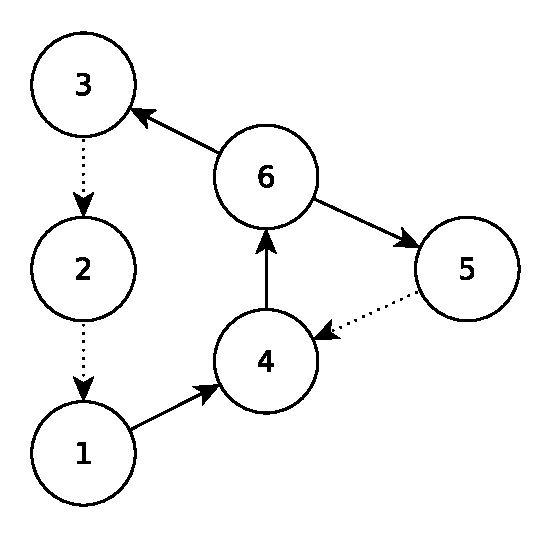
\includegraphics[scale=0.4]{\string~/gitsky/phd/gfx/woodin_equivalences.pdf}
    \caption{Proof strategy of Proposition \ref{prop.woodin}, dotted lines are trivial implications.}
  \end{center}
\end{figure}

\proof{
  Firstly note that $(iii)\Rightarrow(ii)\Rightarrow(i)$ and $(v)\Rightarrow(iv)$ are simply by definition.
  
  \qquad\framebox{$(i)\Rightarrow(iv)$} Assume $\delta$ is virtually woodin, and fix a function $f\colon\delta\to\delta$. Let $\kappa<\delta$ be virtually $({<}\delta, f)$-strong and let $\theta:=\sup_{\alpha\leq\kappa}f(\alpha){+}1$. Then there's a generic elementary embedding $\pi\colon (H_\theta^V, \in, f\cap H_\theta^V) \to (\M, \in, f^+)$ where $f^+\restr\kappa = f\restr\kappa$, $\M\subset V$ and $\pi(\kappa)>\theta$. We firstly want to show that $\kappa$ is a closure point for $f$, so let $\alpha<\kappa$. Then
  \eq{
    f(\alpha)=f^+(\alpha)=\pi(f)(\alpha)=\pi(f)(\pi(\alpha))=\pi(f(\alpha)),
  }

  so $\pi$ fixes $f(\alpha)$ for every $\alpha<\kappa$. Now, if $\kappa$ wasn't a closure point for $f$ then, letting $\alpha<\kappa$ be the least such that $f(\alpha)\geq\kappa$,
  \eq{
    \theta > f(\alpha) = \pi(f(\alpha)) > \theta,
  }

  a contradiction. Note that we used that $\pi(\kappa)>\theta$ here, so this argument wouldn't work if we had only assumed $\delta$ to be virtually prewoodin. Lastly, $\theta$-strongness implies that $H_\theta^V\subset\M$, and $\M\subset V$ holds by assumption.

  \qquad \framebox{$(iv)\Rightarrow(vi)$} Assume $(iv)$ holds, let $f\colon\delta\to\delta$ be given and define $g\colon\delta\to\delta$ as $g(\alpha):=(2^{<f(\alpha)})^+$. By $(iv)$ there's a $\kappa<\delta$ which is a closure point of $g$ and there's a regular $\theta\in(\kappa, \delta)$ and a generic elementary $\pi\colon H_\theta^V\to\M$ with $\crit\pi=\kappa$, $H_\theta^V\subset\M$, $\M\subset V$ and $\theta=\pi(f\restr\kappa)(\kappa)$. We want to find a regular $\bar\theta<\kappa$ and another elementary embedding $\sigma\colon H_{\bar\theta}^V\to H_\theta^V$ with $\sigma(\crit\sigma)=\kappa$, $f(\crit\sigma)=\bar\theta$ and $f\restr\kappa\in\ran\sigma$.

  \qquad Note that $\M\subset V$ and $H_\theta^V\subset\M$ implies that $H_\theta^V = H_\theta^{\M}$, so that both $H_\theta^V$ and $H_{\pi(\theta)}^{\M}$ are elements of $\M$ (we introduced $g$ to ensure that $\pi(\theta)$ makes sense). An application of Countable Embedding Absoluteness \ref{lemm.ctblabs} then yields that $\M$ has a generic elementary embedding $\pi^*\colon H_\theta^{\M}\to H_{\pi(\theta)}^{\M}$ such that $\crit\pi^*=\kappa$, $\pi^*(\kappa)=\pi(\kappa)$ and $\pi(f\restr\kappa)\in\ran\pi^*$.

  \qquad By elementarity of $\pi$, $H_\theta^V$ has an ordinal $\bar\theta<\kappa$ and a generic elementary embedding $\sigma\colon H_{\bar\theta}^V\to H_\theta^V$ with $\sigma(\crit\sigma)=\kappa$, $f\restr\kappa\in\ran\sigma$ and $\bar\theta = f(\crit\sigma)$, which is what we wanted to show.

  \qquad \framebox{$(vi)\Rightarrow(v)$} Assume $(vi)$ holds and let $f\colon\delta\to\delta$ be given. Define $g\colon\delta\to\delta$ as $g(\alpha):=(2^{<f(\alpha)})^+$, so that by $(vi)$ there exist regular $\bar\kappa<\bar\theta<\kappa<\theta$ such that $\kappa$ is a closure point for $g$ and there exists a generic elementary embedding $\pi\colon H_{\bar\theta}^V\to H_\theta^V$ with $\crit\pi = \bar\kappa$, $\pi(\bar\kappa)=\kappa$, $g(\bar\kappa)=\bar\theta$ and $g\restr\kappa\in\ran\pi$.

  \qquad Now, following the $(iii)\Rightarrow(ii)$ direction in the proof of Theorem \ref{theo.rem} we get a transitive $\M\in H_{g(\bar\kappa)}^V$ closed under ${<}f(\bar\kappa)$-sequences, and $H_{g(\bar\kappa)}^V$ has a generic elementary embedding $\sigma\colon H_{f(\bar\kappa)}^V\to\M$ with $\crit\sigma=\bar\kappa$ and $\sigma(\bar\kappa)=\kappa> f(\bar\kappa)$. In other words, $\bar\kappa$ is virtually $f(\bar\kappa)$-supercompact in $H_{\bar\theta}^V$. Elementarity of $\pi$ then implies that $\kappa$ is virtually $\pi(f)(\kappa)$-supercompact in $H_\theta^V$, which is what we wanted to show.

  \qquad \framebox{$(vi)\Rightarrow(iii)$} Let $C$ be the club of all $\alpha$ such that $(H_\alpha^V,\in, A\cap H_\alpha^V)\prec(H_\delta^V,\in,A)$. Let $f\colon\delta\to\delta$ be given as $f(\alpha)=\bra{\alpha_0,\alpha_1}$ with $\bra{-,-}$ being the G\"odel pairing function, where $\alpha_0$ is the first limit of elements of $C$ above $\alpha$ and the $\alpha_1$'s are chosen such that $\{\alpha_1\mid\alpha<\beta\}$ encodes $A\cap\beta$. This definition makes sense since $\delta$ is inaccessible by Proposition \ref{prop.virtit}.

  \qquad Let $\kappa<\delta$ be a closure point of $f$ such that there are regular cardinals $\bar\theta<\kappa$, $\theta>\kappa$ and a generic elementary embedding $\pi\colon H_{\bar\theta}^V\to H_\theta^V$ such that $\pi(\crit\pi)=\kappa$, $f(\crit\pi)=\bar\theta$, and $f\restr\kappa\in\ran\pi$. We claim that $\bar\kappa:=\crit\pi$ is virtually $({<}\delta, A)$-extendible. To see this, it suffices by the definition of $C$ to show that
  \eq{
    (H_\kappa^V,\in,A\cap H_\kappa^V)\models\godel{\text{$\bar\kappa$ is virtually $(A\cap H_\kappa)$-extendible}}, \tag*{$(1)$}
  }

  since $\kappa\in C$ because it is a closure point of $f$. Let $\beta := \min(C-\bar\kappa) < \bar\theta$ and note that $\beta$ exists as $f(\bar\kappa)=\bar\theta$ so the definition of $f$ says that $\bar\theta$ is a limit of elements of $C$ above $\bar\kappa$. It then holds that $(H_{\bar\kappa}^V,\in,A\cap H_{\bar\kappa}^V) \prec (H_\beta^V,\in,A\cap H_\beta^V)$ as both $\bar\kappa$ and $\beta$ are elements of $C$. Since $f$ encodes $A$ in the manner previously described and $\pi^{-1}(f)\restr\bar\kappa=f\restr\bar\kappa$, we get that $\pi(A\cap H_{\bar\kappa}^V) = A\cap H_\kappa^V$ and thus
  \eq{
    (H_\kappa^V,\in,A\cap H_\kappa^V) \prec (H_{\pi(\beta)}^V,\in,A^*) \tag*{$(2)$}
  }

  for $A^* := \pi(A\cap H_\beta^V)$. Now, as $(H_\gamma^V,\in, A\cap H_\gamma^V)$ and $(H_{\pi(\gamma)}^V,\in,A^*\cap H_{\pi(\gamma)}^V)$ are elements of $H_{\pi(\beta)}^V$ for every $\gamma<\kappa$, Countable Embedding Absoluteness \ref{lemm.ctblabs} implies that $H_{\pi(\beta)}^V$ sees that $\bar\kappa$ is virtually $({<}\kappa, A^*)$-extendible, which by $(2)$ then implies $(1)$, which is what we wanted to show.
}

\rema{
  The above proof shows that the $\M\subset V$ assumptions can be replaced by ``sufficient'' agreement between $\M$ and $V$: for $(i)$-$(iii)$ this means that $H_\theta^{\M}=H_\theta^V$ whenever $\M$ is the codomain of a virtual $(\theta,A)$-strong/supercompact/extendible embedding, and in $(iv)$-$(v)$ this means that $H_{\pi(f)(\kappa)}^{\M} = H_{\pi(f)(\kappa)}^V$. The same thing holds in the ``lightface'' setting of Theorem \ref{theo.rem}.
}

We will now step away from the woodins for a little bit, and introduce the vop\v enkas. In anticipation of the next section we will work with the class-sized version here, but all the following results work equally well for inaccessible virtually vop\v enka cardinals\footnote{Note however that we have to require inaccessibility here: see \cite{WilsonVopenka} for an analysis of the singular virtually vop\v enka cardinals.\todo[inline]{Redundant; mention this properly above}}.

\defi[\gbc]{
  The \textbf{Generic Vop\v enka Principle} (\gvp) states that for any class $C$ consisting of structures in a common language, there are distinct $\M,\N\in C$ and a generic elementary embedding $\pi\colon\M\to\N$.
}

We will be using a standard variation of \gvp\, involving the following \textit{natural sequences}.

\defi[\gbc]{
  Say that a class function $f\colon\on\to\on$ is an \textbf{indexing function} if it satisfies that $f(\alpha)>\alpha$ and $f(\alpha)\leq f(\beta)$ for all $\alpha<\beta$.
}

\defi[\gbc]{
  Say that an $\on$-sequence $\bra{\M_\alpha\mid\alpha<\on}$ is \textbf{natural} if there exists an indexing function $f\colon\on\to\on$ and unary relations $R_\alpha\subset V_{f(\alpha)}$ such that $\M_\alpha = (V_{f(\alpha)}, \in, \{\alpha\}, R_\alpha)$ for every $\alpha$. Denote this indexing function by $f^{\vec\M}$ and the unary relations as $R_\alpha^{\vec\M}$.
}

The following Theorem \ref{theo.vopwood} is then the main theorem of this section. Firstly it shows that inaccessible cardinals are virtually vop\v enka iff they are virtually prewoodin, but also that adding the ``virtually'' adverb doesn't do anything in this context, in contrast to Theorem \ref{theo.virtualsep}. 

\theo[\gbc, Dimopoulos-Gitman-N.][theo.vopwood]{
  The following are equivalent:
  \begin{enumerate}
    \item \gvp\ holds;
    \item For any natural $\on$-sequence $\vec\M$ there exists a generic elementary embedding $\pi\colon\M_\alpha\to\M_\beta$ for some $\alpha<\beta$;
    \item $\on$ is virtually prewoodin;
    \item $\on$ is faintly prewoodin.
  \end{enumerate}
}
\proof{
  $(i)\Rightarrow(ii)$ and $(iii)\Rightarrow(iv)$ are trivial.
  
  \qquad $(iv)\Rightarrow(i)$: Assume $\on$ is faintly prewoodin and fix some $\on$-sequence $\vec\M:=\bra{\M_\alpha\mid\alpha<\on}$ of structures in a common language. Let $\kappa$ be $({<}\on,\vec\M)$-prestrong and fix some regular $\theta>\kappa$ satisfying that $\M_\alpha\in H_\theta^V$ for every $\alpha<\theta$, and fix a generic elementary embedding
  \eq{
    \pi\colon(H_\theta^V, \in, \vec\M) \to (\N, \in, \M^*)
  }

  with $H_\theta^V\subset\N$ and $\vec\M\cap H_\theta^V=\M^*\cap H_\theta^V$. Set $\kappa:=\crit\pi$.

  \qquad We have that $\pi\restr\M_\kappa\colon\M_\kappa\to\M^*_{\pi(\kappa)}$, but we need to reflect this embedding down below $\theta$ as we don't know whether $\M_{\pi(\kappa)}^*$ is on the $\vec\M$ sequence. Working in the generic extension, we have
  \eq{
    \N\models\exists\bar\kappa<\pi(\kappa)\exists\dot\sigma\in V^{\col(\omega, \M_{\bar\kappa}^*)}\colon \godel{\text{$\dot\sigma\colon \M^*_{\bar\kappa}\to\M^*_{\pi(\kappa)}$ is elementary}}.
  }

  Here $\kappa$ realises $\bar\kappa$ and $\pi\restr\M_\kappa$ realises $\sigma$. Note that $\M^*_\kappa = \M_\kappa$ since we ensured that $\M_\kappa\in H_\theta^V$ and we are assuming that $\vec\M\cap H_\theta^V = \M^*\cap H_\theta^V$, so the domain of $\sigma$ ($=\pi\restr\M_\kappa$) \textit{is} $\M_\kappa^*$ --- also note that $\sigma$ exists in a $\col(\omega,\M_\kappa)$ extension of $\N$ by an application of Countable Embedding Absoluteness \ref{lemm.ctblabs}. Now elementarity of $\pi$ implies that
  \eq{
    H_\theta^V\models\exists\bar\kappa<\kappa\exists\dot\sigma\in V^{\col(\omega, \M_{\bar\kappa})}\colon \godel{\text{$\dot\sigma\colon \M_{\bar\kappa}\to\M_{\kappa}$ is elementary}},
  }

  which is upwards absolute to $V$, from which we can conclude that $\sigma\colon\M_{\bar\kappa}\to\M_\kappa$ witnesses that \gvp\ holds.

  

  \qquad $(ii)\Rightarrow(iii)$: Assume $(ii)$ holds and assume that $\on$ is not virtually prewoodin, which means that there exists some class $A$ such that there are no virtually $A$-prestrong cardinals. This allows us to define a function $f\colon\on\to\on$ as $f(\alpha)$ being the least regular $\eta>\alpha$ such that $\alpha$ is not virtually $(\eta,A)$-prestrong.

  \qquad We also define $g\colon\on\to\on$ as taking $\alpha$ to the least strong limit cardinal above $\alpha$ which is a closure point for $f$. Note that $g$ is an indexing function, so we can let $\vec\M$ be the natural sequence induced by $g$ and $R_\alpha := A\cap H_{g(\alpha)}^V$. $(ii)$ supplies us with $\alpha<\beta$ and a generic elementary embedding\footnote{Note that $V_{g(\alpha)}=H_{g(\alpha)}^V$ since $g(\alpha)$ is a strong limit cardinal.}
  \eq{
    \pi\colon(H_{g(\alpha)}^V,\in,A\cap H_{g(\alpha)}^V)\to (H_{g(\beta)}^V, \in, A\cap H_{g(\beta)}^V).
  }

  Since $g(\alpha)$ is a closure point for $f$ it holds that $f(\crit\pi)<g(\alpha)$, so fixing a regular $\theta\in(f(\crit\pi), g(\alpha))$ we get that $\crit\pi$ is virtually $(\theta, A)$-prestrong, contradicting the definition of $f$. Hence $\on$ is virtually prewoodin.
}


\subsection{Weak Vop\v enka}

\todo[inline]{Scrap this section?}

We now move to a \textit{weak} variant of \gvp, introduced in a category-theoretic context in \cite{AdamekRosicky}. It starts with the following equivalent characterisation of \gvp, which is the virtual analogue of the characterisation shown in \cite{AdamekRosicky}.

\lemm[\gbc, Virtualised Ad\' amek-Rosick\' y][lemm.adaros]{
  $\gvp$ is equivalent to there \textit{not} existing an $\on$-sequence of first-order structures $\bra{\M_\alpha\mid\alpha<\on}$ satisfying that\footnote{This is equivalent to saying that $\on$, viewed as a category, can't be fully embedded into the category \textsf{Gra} of graphs, which is how it's stated in \cite{AdamekRosicky}.}
  \begin{enumerate}
    \item \gvp\
    \item There is not a natural $\on$-sequence $\bra{\M_\alpha\mid\alpha<\on}$ satisfying that
      \begin{itemize}
        \item there is a generic homomorphism $\M_\alpha\to\M_\beta$ for every $\alpha\leq\beta$, which is unique in all generic extensions;
        \item there is \textit{no} generic homomorphism $\M_\beta\to\M_\alpha$ for any $\alpha<\beta$.
      \end{itemize}
    \item There is not a natural $\on$-sequence $\bra{\M_\alpha\mid\alpha<\on}$ satisfying that
      \begin{itemize}
        \item there is a homomorphism $\M_\alpha\to\M_\beta$ in $V$ for every $\alpha\leq\beta$, which is unique in all generic extensions;
        \item there is \textit{no} generic homomorphism $\M_\beta\to\M_\alpha$ for any $\alpha<\beta$.
      \end{itemize}
  \end{enumerate}
}
\proof{
  Note that the only difference between $(ii)$ and $(iii)$ is that the homomorphism exists in $V$, making $(ii)\Rightarrow(iii)$ trivial.

  \qquad $(iii)\Rightarrow(i)$: Assume that \gvp\ fails, meaning by Theorem \ref{theo.vopwood} that we have a natural $\on$-sequence $\vec\M_\alpha$ such that, in every generic extension, there's no homomorphism between any two disctinct $\M_\alpha$'s. Define an $\on$-sequence $\bra{\N_\kappa\mid\kappa\in\Card}$ as
\eq{
  \N_\kappa:=\coprod_{\xi\leq\kappa}\M_\xi= \{(x,\xi)\mid\xi\leq\kappa\land\xi\in\Card\land x\in\M_\xi\},\footnote{$\coprod$ is the ``model-theoretic union'', also known as the coproduct.}
}

  with a unary relation $R^*$ given as $R^*(x, \xi)$ iff $\M_\xi\models R(x)$ and a binary relation $\sim^*$ given as $(x,\xi)\sim^*(x', \xi')$ iff $\xi=\xi'$. Whenever we have a homomorphism $f\colon\N_\kappa\to\N_\lambda$ we then get an induced homomorphism $\tilde f\colon\M_0\to\M_\xi$, given as $\tilde f(x) := f(x, 0)$, where $\xi\leq\kappa$ is given by preservation of $\sim^*$.

  \qquad For any two cardinals $\kappa<\lambda$ we have a homomorphism $j_{\kappa\lambda}\colon\N_\kappa\to\N_\lambda$ in $V$, given as $j_{\kappa\lambda}(x, \xi) := (x,\xi)$. This embedding must also be the \textit{unique} such embedding in all generic extensions, as otherwise we get a generic homomorphism between two distinct $\M_\alpha$'s. Furthermore, there can't be any homomorphism $\N_\lambda\to\N_\kappa$ as that would also imply the existence of a generic homomorphism between two distinct $\M_\alpha$'s.

\qquad $(i)\Rightarrow(ii)$: Assume that we have an $\on$-sequence $\vec\M_\alpha$ as in the theorem, with generic homomorphisms $j_{\alpha\beta}\colon\M_\alpha\to\M_\beta$ that are unique in all generic extensions for every $\alpha\leq\beta$, with no generic homomorphisms going the other way.

\qquad We first note that we can for every $\alpha\leq\beta$ choose the $j_{\alpha\beta}$ in a $\col(\omega,\M_\alpha)$-extension, by a proof similar to the proof of Lemma \ref{lemm.ctblabs} and using the uniqueness of $j_{\alpha\beta}$. Next, fix a proper class $C\subset\on$ such that $\alpha\in C$ implies that
\eq{
  \sup_{\xi\in C\cap\alpha}\abs{\M_\xi}^V<\abs{\M_\alpha}^V.
}

and note that this implies that $V[g]\models\abs{\M_\xi}<\abs{\M_\alpha}$ for every $V$-generic $g\subset\col(\omega,\M_\xi)$. This means that for every $\alpha\in C$ we may choose some $\eta_\alpha\in\M_\alpha$ which is \textit{not} in the range of any $j_{\xi\alpha}$ for $\xi<\alpha$. But now define first-order structures $\bra{\N_\alpha\mid\alpha\in C}$ as $\N_\alpha := (\M_\alpha, \eta_\alpha)$. Then, by our assumption on the $\M_\alpha$'s and construction of the $\N_\alpha$'s, there can be no generic homomorphism between any two distinct $\N_\alpha$, showing that \gvp\ fails.
}

  Note that the proof of the above lemma shows that we without loss of generality may assume that the generic homomorphism in $(i)$ exists in $V$, which we record here:

\qlemm[\gbc, Virtualised Ad\' amek-Rosick\' y][lemm.adaros2]{
  $\gvp$ is equivalent to there \textit{not} existing an $\on$-sequence of first-order structures $\bra{\M_\alpha\mid\alpha<\on}$ satisfying that\footnote{This is equivalent to saying that $\on$, viewed as a category, can't be fully embedded into the category \textsf{Gra} of graphs, which is how it's stated in \cite{AdamekRosicky}.}
  \begin{enumerate}
    \item there is a homomorphism $\M_\alpha\to\M_\beta$ in $V$ for every $\alpha\leq\beta$, which is unique in all generic extensions;
    \item there is \textit{no} generic homomorphism $\M_\beta\to\M_\alpha$ for any $\alpha<\beta$.
  \end{enumerate}
}

The \textit{weak} version of \gvp\ is then simply ``flipping the arrows around'' in the above characterisation of \gvp.

\defi[\gbc]{
  \textbf{Generic Weak Vop\v enka's Principle} (\gwvp) states that there does \textit{not} exist an $\on$-sequence of first-order structures $\bra{\M_\alpha\mid\alpha<\on}$ such that
  \begin{itemize}
    \item there is a generic homomorphism $\M_\beta\to\M_\alpha$ for every $\alpha\leq\beta$, which is unique in all generic extensions;
    \item there is \textit{no} generic homomorphism $\M_\alpha\to\M_\beta$ for any $\alpha<\beta$.
  \end{itemize}
}

Denoting the corresponding non-generic principle by \wvp\, \cite{WilsonWVP} showed the following.

\theo[Wilson]{
  \wvp\ is equivalent to $\on$ being a Woodin cardinal.
}

Given our \ref{theo.vopwood} we may then suspect that in the virtual world these two are equivalent, which indeed turns out to be the case. We will be roughly following the argument in \cite{WilsonWVP}, but we have to diverge from it at several points in which they're using the fact that they're working with class-sized elementary embeddings. 

\qquad Indeed, in that paper they establish a correspondence between elementary embeddings and certain homomorphisms, a correspondence we won't achieve here. Proving that the elementary embeddings we \textit{do} get are non-trivial seems to furthermore require extra assumptions on our structures. Let's begin.

\qquad Define for every strong limit cardinal $\lambda$ and $\Sigma_1$-formula $\varphi$ the relations
\eq{
  R^\varphi &:= \{x\in V\mid (V,\in)\models\varphi[x]\}\\
  R^\varphi_\lambda&:= \{x\subset H_\lambda^V\mid \exists y\in R^\varphi\colon y\cap H_\lambda^V = x\}
}

and given any class $A$ define the structure
\eq{
  \p_{\lambda,A} := (H_{\lambda^+}^V,R^\varphi_\lambda, \{\lambda\}, A\cap H_\lambda^V)_{\varphi\in\Sigma_1}.
}

Say that a homomorphism $h\colon\p_{\lambda,A}\to\p_{\eta,A}$ is \textbf{trivial} if $h(x)\cap H_\eta^V = x\cap H_\eta^V$ for every $x\in H_{\lambda^+}^V$. Note that $h$ can only be trivial if $\eta\leq\lambda$ since $h(\lambda)=\eta$.

\lemm[\gbc, Gitman-N.][lemm.hom]{
  Let $\lambda$ be a singular strong limit cardinal, $\eta$ a strong limit cardinal and $A\subset V$ a class. If there exists a non-trivial generic homomorphism $h\colon\p_{\lambda,A}\to\p_{\eta,A}$ then there's a non-trivial generic elementary embedding
  \eq{
    \pi\colon(H_{\lambda^+}^V,\in,A\cap H_\lambda^V)\to(\M, \in, B)
  }

  for some transitive $\M$ such that, letting $\nu := \min\{\lambda,\eta\}$, it holds that $H_\nu^V\subset\M$, $A\cap H_\nu^V = B\cap H_\nu^V$ and $\crit\pi<\nu$.
}
\proof{
  Assume that we have a non-trivial homomorphism $h\colon\p_{\lambda,A}\to\p_{\eta,A}$ in a forcing extension $V[g]$, define in $V[g]$ the set
  \eq{
    \M^* := \{\bra{b,f} \mid b\in [H_\nu]^{<\omega}\land f\in H_{\lambda^+}^V\land f\colon H_\lambda^V\to H_\lambda^V\},
  }

  and define the relation $\in^*$ on $\M^*$ as
  \eq{
    \bra{b_0,f_0} \in^* \bra{b_1, f_1} \quad\text{iff}\quad b_0b_1\in h(\{xy\in[H_\lambda^V]^{<\omega}\mid f_0(x)\in f_1(y)\}).
  }

  \clai{
    $\in^*$ is wellfounded.
  }

  \cproof{
    Assume not and let $\cdots\in^*\bra{b_1,f_1}\in^*\bra{b_0,f_0}$ be an $\in^*$-decreasing chain, which by definition means that, for every $n<\omega$,
    \eq{
      b_{n+1}b_n\in h(\{xy\in[H_\lambda^V]^{<\omega}\mid f_{n+1}(x)\in f_n(y)\}). \tag*{$(1)$}
    }

    Define the relation $R(v_0,v_1,v_2)$ on $H_\lambda^V$ as
    \eq{
      R(X,f,g)\text{ iff } X = \{xy\in [H_\lambda^V]^{<\omega}\mid f(x) \in g(y)\}.
    }

    This relation is equal to $R^\varphi_\lambda$ for some $\varphi$, so $h$ moves $\bra{X,f,g}\in R^\varphi_\lambda$ to
    \eq{
      \bra{h(X),h(f),h(g)}\in R^\varphi_\eta,
    }

    meaning that
    \eq{
      h(\{xy\in [H_\lambda^V]^{<\omega}\mid f_{n+1}(x)\in f_n(y)\}) = \{xy\in [H_\eta^V]^{<\omega}\mid f_{n+1}^*(x)\in f_n^*(y)\}
    }

    for some $f_n^*$ such that $f_n^*\cap H_\eta^V= h(f_n)$ for all $n<\omega$. But now $(1)$ implies that
    \eq{
      b_{n+1}b_n\in\{xy\in [H_\eta^V]^{<\omega}\mid f_{n+1}^*(x)\in f_n^*(y)\}
    }

    and so $h(f_{n+1})(x) = f_{n+1}^*(x)\in f_n^*(y) = h(f_n)(y)$, giving an $\in$-decreasing sequence in $V[g]$ using transitivity of $H_\eta^V$, a contradiction!

    \qquad Hence $\in^*$ is wellfounded.
  }

  $\M^*$ is a set, so $\in^*$ is trivially set-like. This means that we can take the transitive collapse $(\M,\in)\cong(\M^*,\in^*)$, and we note that $\M = \{[b,f]\mid\bra{b,f}\in\M^*\}$, where $[b,f] := \{[\bar b, \bar f]\mid\bra{\bar b, \bar f}\in^*\bra{b,f}\}$.

  \qquad We now get a version of \L o\' s' Theorem whose proof is straight-forward, using that $h$ preserves all $\Sigma_1$-relations and that $H_\lambda^V\models\zfc^-$.

  \clai{
    For every formula $\varphi(v_1,\dots,v_n)$ and every $[b_1,f_1],\dots,[b_n,f_n]\in\M$ the following are equivalent:
    \begin{enumerate}
      \item $(\M,\in)\models\varphi[[b_1,f_1],\dots,[b_n,f_n]]$;
      \item $b_1\cdots b_n\in h(\{a_1\cdots a_n\mid\p_{\lambda,A}\models\varphi[f_1(a_1),\dots,f_n(a_n)]\})$.
    \end{enumerate}
  }
  
  \cproof{
    The proof is straightforward, using that $h$ preserves $\Sigma_1$-relations. We prove this by induction on $\varphi$. If $\varphi$ is $v_i\in v_j$ then we have that
    \eq{
      &(\M,\in)\models\varphi[[b_1,f_1],\dots,[b_n,f_n]]\\
      \Leftrightarrow&[b_i,f_i]\in[b_j,f_j]\\
      \Leftrightarrow&\bra{b_i,f_i}\in^*\bra{b_j,f_j}\\
      \Leftrightarrow&b_ib_j \in h(\{a_ia_j\in[H_\lambda^V]^{<\omega}\mid f_i(a_i)\in f_j(a_j)\})\\
      \Leftrightarrow&b_1\cdots b_n\in h(\{a_1\cdots a_n\mid f_i(a_i)\in f_j(a_j)\})\\
      \Leftrightarrow&b_1\cdots b_n\in h(\{a_1\cdots a_n\mid\p_{\lambda,A}\models\varphi[f_1(a_1),\dots,f_n(a_n)]\}).
    }

    If $\varphi$ is $\psi\land\chi$ then
    \eq{
      &(\M,\in)\models\varphi[[b_1,f_1],\dots,[b_n,f_n]]\\
      \Leftrightarrow&(\M,\in)\models\psi[[b_1,f_1],\dots,[b_n,f_n]]\land\chi[[b_1,f_1],\dots,[b_n,f_n]]\\
      \Leftrightarrow&b_1\cdots b_n\in h(\{a_1\cdots a_n\mid\p_{\lambda,A}\models\psi[f_1(a_1),\dots,f_n(a_n)]\})\cap\\ &\hspace{1.6cm} h(\{a_1\cdots a_n\mid\p_{\lambda,A}\models\chi[f_1(a_1),\dots,f_n(a_n)]\})\\
      \Leftrightarrow&b_1\cdots b_n\in h(\{a_1\cdots a_n\mid\p_{\lambda,A}\models\varphi[f_1(a_1),\dots,f_n(a_n)]\}).
    }

    If $\varphi$ is $\lnot\psi$ then
    \eq{
      &(\M,\in)\models\varphi[[b_1,f_1],\dots,[b_n,f_n]]\\
      \Leftrightarrow&(\M,\in)\models\lnot\psi[[b_1,f_1],\dots,[b_n,f_n]]\\
      \Leftrightarrow&(\M,\in)\not\models\psi[[b_1,f_1],\dots,[b_n,f_n]]\\
      \Leftrightarrow&b_1\cdots b_n\notin h(\{a_1\cdots a_n\mid\p_{\lambda,A}\models\psi[f_1(a_1),\dots,f_n(a_n)]\})\\
      \Leftrightarrow&b_1\cdots b_n\in h(\{a_1\cdots a_n\mid\p_{\lambda,A}\models\varphi[f_1(a_1),\dots,f_n(a_n)]\}).
    }

    Finally, if $\varphi$ is $\exists x\psi$ then
    \eq{
      &(\M,\in)\models\varphi[[b_1,f_1],\dots,[b_n,f_n]]\\
      \Leftrightarrow&(\M,\in)\models\exists x\psi[x, [b_1,f_1],\dots,[b_n,f_n]]\\
      \Leftrightarrow&\exists\bra{b,f}\in\M^*\colon(\M,\in)\models\psi[[b,f], [b_1,f_1],\dots,[b_n,f_n]]\\
      \Leftrightarrow&\exists\bra{b,f}\in\M^*\colon bb_1\cdots b_n\in h(\{aa_1\cdots a_n\mid\p_{\lambda,A}\models\psi[f(a), f_1(a_1),\dots,f_n(a_n)]\})\\
      \Leftrightarrow&b_1\cdots b_n\in h(\{a_1\cdots a_n\mid\p_{\lambda,A}\models\varphi[f_1(a_1),\dots,f_n(a_n)]\}).
    }

    This finishes the proof.
  }

  Next up, we have the following standard lemma, which implies that $H_\eta^V\subset\M$:

  \clai{
    \label{clai.pr}
    For all $y\in H_\eta^V$ we have $y = [\bra{y},\text{pr}]$, where $\text{pr}(\bra{x}) := x$.
  }

  \cproof{
    We prove this by $\in$-induction on $y\in H_\eta^V$, so suppose that $y' = [\bra{y'},\text{pr}]$ for every $y'\in y$, which implies that $y\subset\M$ by transitivity of $\M$. We then get that, for every $[b,f]\in\M$,
    \eq{
      [b,f]\in [\bra{y},\text{pr}] &\Leftrightarrow b\bra{y}\in h(\{a\bra{x}\mid f(a)\in\text{pr}(\bra{x})\})\\
      &\Leftrightarrow \exists y'\in y\colon b\bra{y'}\in h(\{a\bra{x}\mid f(a)=x\})\\
      &\Leftrightarrow \exists y'\in y\colon [b,f] = [\bra{y'},\text{pr}] = y'\\
      &\Leftrightarrow [b,f]\in y,
    }

    showing that $y = [\bra{y},\text{pr}]$.
  }

  Now define
  \eq{
    B := \{[b,f]\in\M\mid b\in h(\{x\in H_\lambda^V\mid f(x)\in A\})\}.
  }
  
  and, in $V[g]$, let $\pi\colon (H_\lambda^V,\in,A\cap H_\lambda^V)\to(\M,\in, B)$ be given as $\pi(x) := [\bra{},c_x]$. 
  
  \clai{
    $\pi$ is elementary.
  }

  \cproof{
     For $x_1,\dots,x_n\in H_\lambda^V$ it holds that
    \eq{
      &(\M,\in, B)\models\varphi[\pi(x_1),\dots,\pi(x_n)]\\
      \Leftrightarrow\ &(\M,\in)\models\varphi[\pi(x_1),\dots,\pi(x_n)]\\
      \Leftrightarrow\ &\bra{}\in h(\{\bra{}\mid\p_{\lambda,A}\models\varphi[x_1,\dots,x_n]\})\\
      \Leftrightarrow\ &(H_{\lambda^+}^V,\in,A\cap H_\lambda^V)\models\varphi[x_1,\dots,x_n]
    }

    and we also get that, for every $x\in H_\lambda^V$,
    \eq{
      x\in A \Leftrightarrow \bra{}\in h(\{a\in H_\lambda^V\mid x\in A\}) \Leftrightarrow \pi(x)\in B,
    }

    which shows elementarity.
  }

  We next need to show that $B\cap H_\nu^V = A\cap H_\nu^V$, so let $x\in H_\nu^V$. 
  Note that $x = [\bra{x}, \text{pr}]$ by Claim \ref{clai.pr}, which means that
  \eq{
    x\in B \Leftrightarrow \bra{x}\in h(\{\bra{y}\in H_\lambda^V\mid y\in A\}) \Leftrightarrow x\in A.
  }

  The last thing we need to show is that $\crit\pi<\nu$. We start with an analogous result about $h$. 

  \clai{
    \label{clai.move}
    There exists some $b\in H_\nu^V$ such that $h(b)\neq b$.
  }
  
  \cproof{
    Assume the claim fails. We now have two cases.\\
    
    \framebox{\textbf{Case 1:} $\lambda\geq\eta$}
    
    \qquad By non-triviality of $h$ there's an $x\in H_{\lambda^+}^V$ such that $h(x)\cap H_\eta^V\neq x\cap H_\eta^V$, which means that there exists an $a\in H_\eta^V$ such that $a\in h(x)\Leftrightarrow a\notin x$.

    \qquad  If $a\in x$ then $\{a\} = h(\{a\}) \subset h(x)$,\footnote{Note that as $h$ preserves $\Sigma_1$ formulas it also preserves singletons and boolean operations.} making $a\in h(x)$, $\contr$, so assume instead that $a\in h(x)$. Since $\eta$ is a strong limit cardinal we may fix a cardinal $\theta<\eta$ such that $a\in H_\theta^V$ and $H_\theta^V\in H_\eta^V$. We then have that\footnote{Note that we're using $\lambda\geq\eta$ here to ensure that $H_\theta^V\in\dom h$.}
    \eq{
      \{a\}\subset h(x)\cap H_\theta^V = h(x)\cap h(H_\theta^V) = h(x\cap H_\theta^V) = x\cap H_\theta^V,
    }

    so that $a\in x$, $\contr$.\\

    \framebox{\textbf{Case 2:} $\lambda<\eta$}

    \qquad In this case we are assuming that $h\restr H_\lambda^V = \id$, but $h(\lambda) = \eta > \lambda$. Since $\lambda$ is singular we can fix some $\gamma<\lambda$ and a cofinal function $f\colon\gamma\to\lambda$. Define the relation
    \eq{
      R = \{(\alpha,\beta,\bar\alpha,\bar\beta,g)\mid\godel{\text{$g$ is a cofinal function $g\colon\alpha\to\beta$}}\land g(\bar\alpha)=\bar\beta\}.
    }

    Then $R(\gamma,\lambda,\alpha,f(\alpha),f)$ holds by assumption for every $\alpha<\gamma$, so that $R$ holds for some $(\gamma^*,\lambda^*,\alpha^*,f(\alpha)^*,f^*)$ such that
    \eq{
      (\gamma^*,\lambda^*,\alpha^*,f(\alpha)^*,f^*)\cap H_\eta^V &= (h(\gamma),h(\lambda),h(\alpha),h(f(\alpha)),h(f)) \\
      &= (\gamma,\eta,\alpha,f(\alpha),h(f)),
    }

     using our assumption that $h$ fixes every $b\in H_\lambda^V$. Since $\gamma$, $\alpha$ and $f(\alpha)$ are transitive and bounded in $H_\lambda^V$ it holds that $h(\gamma)=\gamma^*$, $h(\alpha)=\alpha^*$ and $h(f(\alpha))=f(\alpha)^*$. Also, since $\dom(f^*)=\gamma=\dom(f)$ we must in fact have that $f^*=h(f)$. But this means that $h(f)\colon\gamma\to\eta$ is cofinal and $\ran(h(f))\subset\lambda$, a contradiction!
  }
  
  To use the above Claim \ref{clai.move} to conclude anything about $\pi$ we'll make use of the following standard lemma.

  \clai{
    \label{clai.pihagreement}
    For any $x\in H_\lambda^V$ it holds that $h(x)\cap H_\eta^V = \pi(x)\cap H_\eta^V$.
  }

  \cproof{
    For any $n<\omega$ and $\bra{a_1,\hdots,a_n}\in[H_\eta^V]^n$ we have that
    \eq{
      &\bra{a_1,\dots,a_n}\in\pi(x)\\
      \Leftrightarrow\ &(\M,\in)\models\bra{a_1,\dots,a_n}\in\pi(x)\\
      \Leftrightarrow\ &(\M,\in)\models\bra{[\bra{a_1},\text{pr}],\dots,[\bra{a_n},\text{pr}]}\in[\bra{},c_x]\\
      \Leftrightarrow\ &\bra{a_1,\hdots,a_n}\in h(\{\bra{x_1,\hdots,x_n}\mid\p_{\lambda,A}\models\bra{x_1,\dots,x_n}\in x\})\\
      \Leftrightarrow\ &\bra{a_1,\dots,a_n}\in h(x),
    }

    showing that $h(x)\cap H_\eta^V = \pi(x)\cap H_\eta^V$.
  }

  Now use Claim \ref{clai.move} to fix a $b\in H_\nu^V$ which is moved by $h$. Claim \ref{clai.pihagreement} then implies that
  \eq{
    \pi(b)\cap H_\eta^V = h(b)\cap H_\eta^V = h(b)\neq b = b\cap H_\eta^V,
  }

  showing that $\pi(b)\neq b$ and hence $\crit\pi<\nu$. This finishes the proof of the lemma.
}


\theo[\gbc, Gitman-N.]{
  \gvp\ is equivalent to \gwvp.
}
\proof{
  $(\Rightarrow)$: Assume \gvp\ holds and \gwvp\ fails, and let $\bra{\M_\alpha\mid\alpha<\on}$ be an $\on$-sequence of first-order structures such that for every $\alpha\leq\beta$ there exists a generic homomorphism
  \eq{
    j_{\beta\alpha}\colon\M_\beta\to\M_\alpha
  }

  in some $V[g]$ which is unique in all generic extensions, with no generic homomorphisms going the other way. Here we may assume, as in the proof of Lemma \ref{lemm.adaros}, that $g\subset\col(\omega,\M_\beta)$. We can then find a proper class $C\subset\on$ such that $\abs{\M_\alpha}^V < \abs{\M_\beta}^V$ for every $\alpha<\beta$ in $C$. By \gvp\ there are then $\alpha<\beta$ in $C$ and a generic homomorphism
  \eq{
    \pi\colon\M_\alpha\to\M_\beta.
  }

  in some $V[h]$, where again we may assume that $h\subset\col(\omega,\M_\alpha)$. But then $\pi\circ j_{\beta\alpha} = \id$ by uniqueness of $j_{\beta\beta} = \id$, which means that $j_{\beta\alpha}$ is injective in $V[g\times h]$ and hence also in $V[g]$. But then $\abs{\M_\beta}^{V[g]}\leq\abs{\M_\alpha}^{V[g]}$, which implies that $\abs{\M_\beta}^V\leq\abs{\M_\alpha}^V$ by the $\abs{\M_\beta}^{+V}$-cc of $\col(\omega,\M_\beta)$, contradicting the definition of $C$.

  \qquad $(\Leftarrow)$: Assume that \gvp\ fails, which by Theorem \ref{theo.vopwood} is equivalent to $\on$ not being faintly prewoodin. This means that there exists a class $A$ such that there are no faintly $A$-prestrong cardinals. We can therefore assign to any cardinal $\kappa$ the least cardinal $f(\kappa)>\kappa$ such that $\kappa$ is not faintly $(f(\kappa),A)$-prestrong.

  \qquad Also define a function $g\colon\on\to\Card$ as taking an ordinal $\alpha$ to the least singular strong limit cardinal above $\alpha$ closed under $f$. Then we're assuming that there's no non-trivial generic elementary embedding
  \eq{
    \pi\colon(H_{g(\alpha)}^V,\in,A\cap H_{g(\alpha)}^V)\to(\M,\in, B)
  }

  with $H_{g(\alpha)}^V\subset\M$ and $B\cap H_{g(\alpha)}^V = A\cap H_{g(\alpha)}^V$. Assume towards a contradiction that for some $\alpha,\beta$ there is a non-trivial generic homomorphism $h\colon\p_{g(\alpha),A}\to\p_{g(\beta), A}$. Lemma \ref{lemm.hom} then gives us a non-trivial generic elementary embedding
  \eq{
    \pi\colon(H_{g(\alpha)}^V,\in,A\cap H_{g(\alpha)}^V)\to(\M, \in, B)
  }

  for some transitive $\M$ such that $H_\nu^V\subset\M$ with $\nu := \min\{g(\alpha),g(\beta)\}$ and $A\cap H_\nu^V = B\cap H_\nu^V$, a contradiction! Therefore every generic homomorphism $h\colon\p_{g(\alpha),A}\to\p_{g(\beta),A}$ is trivial. Since there is a unique trivial homomorphism when $\alpha\geq\beta$ and no trivial homomorphism when $\alpha<\beta$ since $g(\alpha)$ is sent to $g(\beta)$, the sequence of structures
  \eq{
    \bra{\p_{g(\alpha),A}\mid \alpha\in\on}
  }

  is a counterexample to \gwvp, which is what we wanted to show.
}


\section{Berkeleys}

Berkeley cardinals was introduced by Woodin at University of California, Berkeley around 1992, and was introduced as a large cardinal candidate that would be inconsistent with \zf. They trivially imply the Kunen inconsistency and are therefore at least inconsistent with \zfc, but that's as far as it currently goes. In the virtual setting the virtually berkeley cardinals, like all the other virtual large cardinals, are simply downwards absolute to $L$. See Appendix \ref{apx.large-cardinals} for a quick overview of what is currently known about the non-virtual Berkeley cardinals.

\qquad It turns out that virtually berkeley cardinals are natural objects, as the main theorem of this section shows that these large cardinals are precisely what separates virtually prewoodins from the virtually woodins, as well as separating virtually vop\v enka cardinals from mahlo cardinals.

\defi{
  Say that a cardinal $\delta$ is \textbf{virtually proto-berkeley} if for every transitive set $\M$ such that $\delta\subset\M$ there exists a generic elementary embedding $\pi\colon\M\to\M$ with $\crit\pi<\delta$.

  \qquad If $\crit\pi$ can be chosen arbitrarily large below $\delta$ then $\delta$ is \textbf{virtually berkeley}, and if $\crit\pi$ can be chosen as an element of any club $C\subset\delta$ we say $\delta$ is \textbf{virtually club berkeley}.
}

Virtually (proto-)berkeley cardinals turn out to be equivalent to their ``boldface'' versions, the proof of which is a straight-forward virtualisation of Lemma 2.1.12 and Corollary 2.1.13 in \cite{Cutolo}.

\prop[Virtualised Cutolo][prop.boldfaceberkeley]{
  If $\delta$ is virtually proto-berkeley then for every transitive set $\M$ such that $\delta\subset\M$ and every subset $A\subset\M$ there exists a generic elementary embedding $\pi\colon(\M,\in,A)\to(\M,\in,A)$ with $\crit\pi<\delta$. If $\delta$ is virtually berkeley then we can furthermore ensure that $\crit\pi$ is arbitrarily large below $\delta$.
}
\proof{
  Let $\M$ be transitive with $\delta\subset\M$ and $A\subset\M$. Let
  \eq{
    \N := \M\cup\{\{\bra{A,x}\mid x\in\M\}\}
  }

  and note that $\N$ is transitive. Further, both $A$ and $\M$ are definable in $\N$ without parameters: $a$ is the first element in the pairs belonging to the set of highest rank, and $\M$ is what remains if we remove the set with the highest rank. But this means that a generic elementary embedding $\pi\colon\N\to\N$ fixes both $\M$ and $a$, giving us a generic elementary $\sigma\colon(\M,\in,A)\to(\M,\in,A)$ with $\crit\sigma=\crit\pi$, yielding the wanted conclusion.
}

The following is a straight-forward virtualisation of the usual definition of the vop\v enka filter (see e.g. \cite{Kanamori}).

\defi[\gbc]{
  Define the \textbf{virtually vop\v enka filter} $F$ on $\on$ as $X\in F$ iff there's a natural $\on$-sequence $\vec\M$ such that $\crit\pi\in X$ for any $\alpha<\beta$ and any generic elementary $\pi\colon\M_\alpha\to\M_\beta$.
}

  Theorem \ref{theo.vopwood} shows that $\emptyset$ is in the virtually vop\v enka filter iff \gvp\ fails, in analogy with the non-virtual case. Normality also holds in the virtual context, as the following proof shows.
  
\lemm[\gbc, Virtualised folklore]{
  The virtually vop\v enka filter is a normal filter.
}
\proof{
  Let $F$ be the virtually vop\v enka filter. We first show that $F$ is actually a filter. If $X\in F$ and $Y\supset X$ then $Y\in F$ simply by definition of $F$. If $X,Y\in F$, witnessed by natural sequences $\vec\M$ and $\vec\N$, then $X\cap Y\in F$ as well, witnessed by the natural sequence $\vec\P$ induced by the indexing function $f^{\vec\P} := \max(f^{\vec\M}, f^{\vec\N})$ and unary relations $R^{\vec\P}_\alpha := \text{Code}(\bra{R^{\vec\M}_\alpha, R^{\vec\N}_\alpha})$. Indeed, if $\pi\colon\P_\alpha\to\P_\beta$ is a generic elementary embedding with critical point $\mu$ then $\mu$ is also the critical point of both $\pi\restr\M_\alpha\colon\M_\alpha\to\M_\beta$ and $\pi\restr\N_\alpha\colon\N_\alpha\to\N_\beta$.
  
  \qquad For normality, let $X\in F^+$ be $F$-positive, where we recall that this means that $X\cap C\neq\emptyset$ for every $C\in F$, and let $f\colon X\to\on$ be regressive. We want to show that $f$ is constant on an $F$-positive set.

  \qquad Assume this fails, meaning that there are natural sequences $\vec\M^\gamma$ for $\gamma$ such that for any generic elementary $\pi\colon\M_\alpha^\gamma\to\M_\beta^\gamma$ satisfies that $f(\crit\pi)\neq\gamma$. Define a new natural sequence $\vec\N$ as induced by the indexing function $g\colon\on\to\on$ given as $g(\alpha):=\sup_{\gamma<\alpha}\rk\M_\alpha^\gamma + \omega$ and unary relations $R_\alpha^{\vec\N}$ given as
\eq{
  R_\alpha^{\vec\N} := \text{Code}(\bra{\bra{\M_\alpha^\gamma\mid\gamma<\alpha}, f\restr\alpha}).
}

Now since $X$ is $F$-positive there exists a generic elementary embedding $\pi\colon\N_\alpha\to\N_\beta$ with $\crit\pi\in X$. As $f(\crit\pi)<\crit\pi$ we get that $\pi(f(\crit\pi))=f(\crit\pi)$, so that we have a generic elementary embedding
\eq{
  \pi\restr\M_\alpha^{f(\crit\pi)}\colon\M_\alpha^{f(\crit\pi)}\to\M_\beta^{f(\crit\pi)},
}

  but this contradicts the definition of $\vec\M^{f(\crit\pi)}$! Thus $F$ is normal.
}

  The reason why we are being careful in showing all these analogous properties for the virtual vop\v enka filter is that not all properties carry over. Indeed, note that uniformity of filters is non-trivial as we're working with proper classes\footnote{This boils down to the fact that the class club filter is not provably normal in \gbc, see \cite{class-fodor}}, and we will see in Theorem \ref{theo.berkeleyequiv} shows that uniformity of this filter is equivalent to there being no virtually berkeley cardinals --- the following lemma is the first implication.

\lemm[\gbc, N.][lemm.vopclub]{
  Assume $\gvp$ and that there are no virtually berkeley cardinals. Then the virtually vop\v enka filter $F$ on $\on$ contains every class club $C$.
}
\proof{
  The crucial extra property we get by assuming that there aren't any virtually berkeleys is that $F$ becomes uniform, i.e. contains every tail $(\delta,\on)\subset\on$. Indeed, assume that $\delta$ is the least cardinal such that $(\delta,\on)\notin F$. Let $M$ be a transitive set with $\delta\subset M$ and $\gamma<\delta$ a cardinal. As $(\gamma,\on)\in F$ by minimality of $\delta$, we may fix a natural sequence $\vec\N$ witnessing this. Let $\vec\M$ be the natural sequence induced by the indexing function $f\colon\on\to\on$ given by
  \eq{
    f(\alpha):=\max(\alpha+1, \delta+1)
  }

and unary relations $R_\alpha := \bra{M, \N_\alpha}$. If $\pi\colon\M_\alpha\to\M_\beta$ is a generic elementary embedding with $\crit\pi\leq\delta$, which exists as $(\delta,\on)\notin F$, then $\pi(R_\alpha)=R_\beta$ implies that $\pi\restr\M\colon\M\to\M$ with $\crit\pi\leq\delta$. We also get that $\crit\pi>\gamma$, as
  \eq{
    \pi\restr\N_{\crit\pi}\colon\N_{\crit\pi}\to\N_{\pi(\crit\pi)}
  }

  is an embedding between two structures in $\vec\N$ and hence $\crit\pi>\gamma$ as $(\gamma,\on)\in F$. This means that $\delta$ is virtually berkeley, a contradiction. Thus $\crit\pi>\delta$, implying that $(\delta,\on)\in F$.

  \qquad Note that the class $C_0\subset\on$ of limit ordinals is in $F$, since it's the diagonal intersection of the tails $(\alpha+1,\on)$. Now let $C\subset\on$ be a class club, and let $C = \{a_\alpha\mid\alpha<\on\}$ be its increasing enumeration. Then $C \supset C_0\cap\triangle_{\alpha<\on}(a_\alpha,\on)$, implying that $C\in F$.
}

\theo[\gbc, N.][theo.prewoodwood]{
  If there are no virtually berkeley cardinals then $\on$ is virtually prewoodin iff $\on$ is virtually woodin.
}
\proof{
  Assume $\on$ is virtually prewoodin, so \gvp\ holds by Theorem \ref{theo.vopwood} and we can let $F$ be the virtually vop\v enka filter. The assumption that there aren't any virtually berkeley cardinals implies that for any class $A$ we not only get a virtually $A$-prestrong cardinal, but we get stationarily many such. Indeed, assume this fails --- we will follow the proof of Theorem \ref{theo.vopwood}.

  \qquad Failure means that there is some class $A$ and some class club $C$ such that there are no virtually $A$-prestrong cardinals in $C$. Since there are no virtually berkeley cardinals, Lemma \ref{lemm.vopclub} imples that $C\in F$, so there exists some natural sequence $\vec\N$ such that whenever $\pi\colon\N_\alpha\to\N_\beta$ is an elementary embedding between two distinct structures of $\vec\N$ it holds that $\crit\pi\in C$. Define $f\colon\on\to\on$ as sending $\alpha$ to the least cardinal $\eta>\alpha$ such that $\alpha$ is not virtually $(\eta,A)$-prestrong if $\alpha\in C$, and set $f(\alpha):=\alpha$ if $\alpha\notin C$. Also define $g\colon\on\to\on$ as $g(\alpha)$ being the least strong limit cardinal in $C$ above $\alpha$ which is a closure point for $f$.

  \qquad Now let $\vec\M$ be the natural sequence induced by $g$ and $R_\alpha := \code(\bra{A\cap H_{g(\alpha)}^V, \N_\alpha})$ and apply \gvp\ to get $\alpha<\beta$ and a generic elementary embedding $\pi\colon\M_\alpha\to\M_\beta$, which restricts to
  \eq{
    \pi\restr(H_{g(\alpha)}^V,\in,A\cap H_{g(\alpha)}^V)\colon(H_{g(\alpha)}^V,\in,A\cap H_{g(\alpha)}^V)\to(H_{g(\beta)}^V,\in,A\cap H_{g(\beta)}^V),
  }
  
  making $\crit\pi$ virtually $(g(\alpha),A)$-prestrong and thus $\crit\pi\notin C$. But as we also get the embedding $\pi\restr\N_\alpha\colon\N_\alpha\to\N_\beta$, we have that $\crit\pi\in C$ by definition of $\vec\N$, $\contr$.

  \qquad Now fix any class $A$ and some large $n<\omega$ and define the class
  \eq{
    C := \{\kappa\in\Card\mid (H_\kappa^V,\in,A\cap H_\kappa^V)\prec_{\Sigma_n}(V,\in,A)\}.
  }

  This is a club and we can therefore find a virtually $A$-prestrong cardinal $\kappa\in C$. Assume that $\kappa$ is not virtually $A$-strong and let $\theta$ be least such that it isn't virtually $(\theta,A)$-strong. Fix a generic elementary embedding
  \eq{
    \pi\colon(H_\theta^V,\in,A\cap H_\theta^V)\to (M,\in,B)
  }

  with $\crit\pi=\kappa$, $H_\theta^V\subset M$, $M\subset V$, $A\cap H_\theta^V = B\cap H_\theta^V$ and $\pi(\kappa)<\theta$.

  \qquad Now $\pi(\kappa)$ is inaccessible, and $(H_{\pi(\kappa)}^V, \in, A\cap H_{\pi(\kappa)}^V) = (H_{\pi(\kappa)}^M,\in,B\cap H_{\pi(\kappa)}^M)$ believes that $\kappa$ is virtually $(A\cap H_{\pi(\kappa)}^V)$-strong as in the proof of Theorem \ref{theo.virtchar}, meaning that $(H_\kappa^V,\in,A\cap H_\kappa^V)$ believes that there is a proper class of virtually $(A\cap H_\kappa^V)$-strong cardinals. But $\kappa\in C$, which means that
  \eq{
    (V,\in,A)\models\godel{\text{There exists a proper class of virtually $A$-strong cardinals}},
  }

  implying that \on\ is virtually woodin.
}

\theo[\gbc, N.][theo.berkgvpmahlo]{
  If there exists a virtually berkeley cardinal $\delta$ then $\gvp$ holds and $\on$ is not mahlo.
}
\proof{
  If $\on$ was Mahlo then there would in particular exist an inaccessible cardinal $\kappa>\delta$, but then $H_\kappa^V\models\godel{\text{there exists a virtually berkeley cardinal}}$, contradicting the incompleteness theorem.

  \qquad To show $\gvp$ we show that $\on$ is virtually prewoodin, which is equivalent by Theorem \ref{theo.vopwood}. Fix therefore a class $A$ --- we have to show that there exists a virtually $A$-prestrong cardinal. For every cardinal $\theta\geq\delta$ there exists a generic elementary embedding 
  \eq{
    \pi_\theta\colon(H_\theta^V,\in,A\cap H_\theta^V)\to(H_\theta^V, \in, A\cap H_\theta^V)
  }

  with $\crit\pi<\delta$. By the pigeonhole principle we thus get some $\kappa<\delta$ which is the critical point of proper class many $\pi_\theta$, showing that $\kappa$ is virtually $A$-prestrong, making $\on$ virtually prewoodin.
}

%The proof of the following theorem is similar to the proof of Theorem 11 in \cite{GitmanHamkins}. Here we improve that result by reducing the assumption from the existence of $0^\sharp$ to the existence of a virtually berkeley cardinal, which we will later see is optimal.
%
%\theo[N.][theo.clubforcing]{
%  If there exists a virtually berkeley cardinal $\delta$ then there is a definable $\gbc$-preserving class forcing notion $\mathbb P$ such that whenever $C\subset\mathbb P$ is class generic over $V$ then
%  \eq{
%    V[C]\models\godel{\text{\gvp\ holds but \on\ is not mahlo}}.
%  }
%}
%\proof{
%  Define $\mathbb P$ as the class forcing adding a class club which avoids the regular cardinals; conditions are closed bounded sets containing no regular cardinals, ordered by end-extension. This forcing is ${\leq}\gamma$-distributive for every ordinal $\gamma$, as it even contains a dense ${\leq}\gamma$-closed subclass: the class of conditions with elements above $\gamma$. This implies that the forcing adds no sets and preserves $\gbc$.\footnote{See e.g. Example 2.2.7 and Corollary 4.3.7 in \cite{Krapf}.}
%
%  \qquad Letting $G\subset\mathbb P$ be $V$-generic, $C:=\bigcup G$ is a class club containing no regular cardinals and $C$ and $G$ are interdefinable, so that $V[C]=V[G]\models\godel{\text{$\on$ is not mahlo}}$. We need to show that $\gvp$ holds in $V[C]$. As $\mathbb P$ is definable we can let $\mathbb P^\theta$ be $H_\theta^V$'s version of $\mathbb P$, for any ordinal $\theta$.
%
%  \clai{
%    For any set $a$ and any natural number $n$ in the meta-theory, let $D_{a,n}\subset\mathbb P$ be the class of $\mathbb P$-conditions $c$ for which there exists an $\omega$-club of cardinals $\theta$ such that
%    \begin{enumerate}
%      \item $H_\theta^V\prec_{\Sigma_n} V$;
%      \item $c\cap\theta\subset\mathbb P^{H_\theta^V}$ is $H_\theta^V$-generic;
%      \item there exists a generic elementary $\pi\colon(H_\theta^V,\in,a,c\cap\theta)\to(H_\theta^V,\in,a,c\cap\theta)$ with critical point below $\delta$.
%    \end{enumerate}
%
%    Then $D_{a,n}$ is a definable dense subclass of $\mathbb P$.
%  }
%
%  \cproof{
%    Let $d$ be a $\mathbb P$-condition --- we're looking for a $\bar c\in D_{a,n}$ extending $d$. Pick a cardinal $\theta>\delta$ above the rank of $a$ of countable cofinality which we may also assume satisfies $H_\theta^V\prec_{\Sigma_n} V$ since this is the case for club many $\theta$. Fix a sequence $\bra{\theta_k\mid k<\omega}$ cofinal in $\theta$. We will now construct $c\subset\theta$ end-extending $d$ which is $H_\theta^V$-generic for $\mathbb P^{H_\theta^V}$. For each $k<\omega$ define the class
%    \eq{
%      D_k := \bigcap\{D\subset\mathbb P^{H_\theta^V}\mid\text{$D$ is open dense and $\Sigma_k^{H_\theta^V}(H_{\theta_k}^V)$}\}.
%    }
%
%    As $\mathbb P^{H_\theta^V}$ is ${\leq}\theta_k$-distributive for all $k<\omega$ we get that all the $D_k$'s are open dense subclasses of $\mathbb P^{H_\theta^V}$. Note that the $D_k$'s also suffice for genericity, as any subclass of $\mathbb P^{H_\theta^V}$ which is definable in $H_\theta^V$ contains some $D_k$. We can therefore build an $H_\theta^V$-generic $g\subset\mathbb P^{H_\theta^V}$ in $V$ such that $c:=\bigcup g$ end-extends $d$, by the usual diagonalisation argument. Since $\delta$ is virtually berkeley, Proposition \ref{prop.boldfaceberkeley} implies that we get a generic elementary embedding
%    \eq{
%      \pi\colon(H_\theta^V,\in,c,a)\to(H_\theta^V,\in,c,a)
%    }
%
%    with $\crit\pi<\delta$. Defining $\bar c:=c\cup\{\theta\}$ we get that $\bar c\in\mathbb P$ because $\theta$ is singular, so we have verified that $\bar c\in D_{a,n}$ end-extends $d$, implying that $D_{a,n}$ is dense in $\mathbb P$.
%  }
%
%  Now we use the claim to show that $\gvp$ holds in $V[C]$, so let's now work in $V[C]$. Fix some $\on$-sequence $\vec\M = \bra{\M_\alpha\mid\alpha<\on}$ of structures in a common language $\mathcal L$. As we are working with definable classes there is some $m<\omega$ and some $\Sigma_m$-formula $\varphi(v,a,C)$ with a set parameter $a\in V$ and a class parameter $C$ defining $\vec\M$.
%
%  \qquad Let $n<\omega$ be much larger than $m$ --- we'll get back to exactly how large later. By the claim we get an $\omega$-club $C_{\text{claim}}$ of cardinals $\theta$ such that the corresponding initial segment of $C$ is in $D_{\bra{a,\mathcal L},n}$. This means that for every $\theta\in C_{\text{claim}}$ there exists a generic elementary embedding
%  \eq{
%    \pi\colon(H_\theta^V,\in,C\cap\theta,a,\mathcal L)\to(H_\theta^V,\in,C\cap\theta,a,\mathcal L),
%  }
%
%  with $\crit\pi<\delta$. 
%
%  \qquad We now claim that $(H_\theta^V, \in, C\cap\theta)\prec_{\Sigma_m}(V, \in, C)$. To see this, suppose that $(H_\theta^V,\in, C\cap\theta)\models\psi(b)$ for some $\Sigma_m$-formula $\psi(v)$ and $b\in H_\theta^V$. This is then forced over $H_\theta^V$ by some $\mathbb P^{H_\theta^V}$-condition $c$, an initial segment of $C\cap\theta$. By choosing $n$ very large, what we meant was that $n$ is large enough to express this forcing relation\footnote{Note that this $n$ works for all the $\theta\in C_{\text{claim}}$ since $H_{\theta_0}^V\prec_{\Sigma_n}H_{\theta_1}^V$ for all $\theta_0,\theta_1\in C_{\text{claim}}$.}, so since $H_\theta^V\prec_{\Sigma_n}V$ we get that $c$ also forces $\psi(b)$ over $V$. So $(V,\in,C)\models\psi(b)$.
%
%  \qquad It follows that the definition of the class $\vec\M$ is absolute to $(H_\theta^V, \in, C\cap\theta)$ since $\vec\M$ was defined by the $\Sigma_m$-formula $\varphi(v,a,C)$, which also means that $\pi$ fixes $\vec\M$ as $\pi$ fixes both $\mathcal L$, $a$ and $C$ by the choice of $\pi$. We then have that $\pi(\M_\kappa)=\pi(\vec\M)_{\pi(\kappa)}=\M_{\pi(\kappa)}$, so that $\pi\restr\M_\kappa\colon\M_\kappa\to\M_{\pi(\kappa)}$ witnesses $\gvp$.
%}

\theo[\gbc, N.][theo.berkeleyequiv]{
  The following are equivalent:
  \begin{enumerate}
    \item \gvp\ implies that $\on$ is mahlo;
    \item $\on$ is virtually prewoodin iff $\on$ is virtually woodin;
    \item There are no virtually berkeley cardinals.
  \end{enumerate}
}
\proof{
  $(iii)\Rightarrow(ii)$ is Theorem \ref{theo.prewoodwood}, and the contraposed version of $(i)\Rightarrow(iii)$ is Theorem \ref{theo.berkgvpmahlo}. For $(ii)\Rightarrow(i)$ note that \gvp\ implies that \on\ is virtually prewoodin by Theorem \ref{theo.vopwood}, which by $(ii)$ means that it's virtually woodin and the usual proof shows that virtually woodins are mahlo\footnote{See e.g. Exercise 26.10 in \cite{Kanamori}.}, showing $(i)$.
}

This also immediately implies the following equiconsistency, as virtually berkeley cardinals have strictly larger consistency strength than virtually woodin cardinals.

\qcoro[N.]{
  The existence of an inaccessible virtually prewoodin cardinal is equiconsistent with the existence of an inaccessible virtually woodin cardinal.
}

\section{Behaviour in canonical inner models}
\label{section.canonical-inner-models}

Most of the cardinals turn out to downwards absolute to most inner models, including $L$:

\prop[][prop.absemb]{
  For any regular uncountable cardinal $\theta$, faintly $\theta$-measurable cardinals are downwards absolute to any transitive class $\U\subset V$ satisfying $\zf^-+\dc$.
}
\proof{
  Let $\kappa$ be faintly $\theta$-measurable, witnessed by a forcing poset $\mathbb P$ and a $V$-generic $g\subset\mathbb P$ such that, in $V[g]$, there's a transitive $\M$ and an elementary embedding $\pi\colon H_\theta^V\to\M$ with $\crit\pi=\kappa$. Fix a transitive class $\U\subset V$ which satisfies $\zf^-+\dc$. Restricting the embedding to $\pi\restr H_\theta^{\U}\colon H_\theta^{\U}\to\N$ we can now apply the Countable Absoluteness Lemma \ref{lemm.ctblabs} to $\pi\restr H_\theta^{\U}$ to get that there exists an embedding $\pi^*\colon H_\theta^{\U}\to\N^*$ in a generic extension of $U$, making $\kappa$ faintly $\theta$-measurable in $\U$.
}

\prop[N.]{
  Let $\theta$ be a regular uncountable cardinal.
  \begin{enumerate}
    \item $L\models\godel{\text{faintly $\theta$-measurables are equivalent to virtually $\theta$-prestrongs}}$.
    \item Assume that $L[\mu]$ exists. It then holds that\\ 
      $L[\mu]\models\godel{\text{faintly $\theta$-measurables are equivalent to virtually $\theta$-measurables}}$.
    \item Assume there is no inner model with a woodin. It then holds that\\
      $K\models\godel{\text{faintly $\theta$-measurables are equivalent to virtually $\theta$-measurables}}$.
  \end{enumerate}
}
\proof{
  For $(i)$ simply note that if $\pi\colon L_\theta\to\N$ is a generic elementary embedding with $\N$ transitive, then by condensation we have that $\N=L_\gamma$ for some $\gamma\geq\theta$, so that $\pi$ also witnesses the virtual $\theta$-prestrongness of $\crit\pi$.

  \qquad $(ii)$: Assume that $V=L[\mu]$ for notational simplicity and let $\kappa$ be faintly $\theta$-measurable, witnessed by a generic elementary embedding $\pi\colon L_\theta[\mu]\to\N$ existing in some generic extension $V[g]$. By condensation we get that $\N=L_\gamma[\overline\mu]$ for some $\gamma\geq\theta$ and $\overline\mu\in V[g]$, but we're not guaranteed that $\overline\mu\in V$ here. Let $\lambda$ be the unique measurable cardinal of $V=L[\mu]$.

  \qquad Note that $\bar\mu$ is a measure on $\pi(\lambda)\geq\lambda$. If $\pi(\lambda)=\lambda$ then $L[\mu]=L[\bar\mu]$ by \cite[Theorem 20.10]{Kanamori} and we trivially get that $\N\subset V$. Assume thus that $\pi(\lambda)>\lambda$, which implies that $L[\bar\mu]$ is an internal iterate of $L[\mu]$ by \cite[Theorem 20.12]{Kanamori}. In particular it then holds that $L[\bar\mu]\subset L[\mu]$, so again we get that $\N\subset V$.

  \qquad $(iii)$: Assume that $V=K=L[\mathcal E]$ and fix a faintly $\theta$-measurable cardinal $\kappa$, witnessed by a generic embedding $\pi\colon L_\theta[\mathcal E]\to\N=L_\gamma[\overline{\mathcal E}]$ in some generic extension $V[g]$. Now coiterate $L[\mathcal E]$ with $L[\overline{\mathcal E}]$, and denote the last models by $\P$ and $\Q$. Since $K=K^{V[g]}$ and as $K$ is universal we get that $\Q\init\P$. Then the $L[\overline{\mathcal E}]$-to-$\Q$ branch did not drop, giving us an iteration embedding $i\colon L[\overline{\mathcal E}]\to\Q$.

  \qquad Note that $\crit i\geq\kappa$ as $\overline{\mathcal E}$ is simply the pointwise image of $\mathcal E$ under $\pi$, so nothing below $\kappa$ is touched and is therefore not used in the comparison either. This means that $\crit(i\circ\pi)=\kappa$, so that $(i\circ\pi)\colon L_\theta[\mathcal E]\to\Q$ witnesses that $\kappa$ is virtually $\theta$-measurable, since $\Q\init\P$ implies that $\Q\subset K$.
}

Note that the proofs of $(ii)$ and $(iii)$ above do not show that $\kappa$ is virtually $\theta$-prestrong, as it might still be the case that $\bar\mu\neq\mu$ or $\bar{\mathcal E}\neq\mathcal E$, so we cannot conclude that $L_\theta[\mu]\subset L_\theta[\bar\mu]$ or $L_\theta[\mathcal E]\subset L_\theta[\overline{\mathcal E}]$. It might still hold however; see Question \ref{ques.prestrong-equivalence}.


\section{Separation results}

Having proving many positive results about the relations between the virtual large cardinals in the previous sections, this section is dedicated to the negatives. More precisely, we will aim to \textit{separate} many of the defined notions (potentially under suitable large cardinal assumptions).

\qquad Our first separation result is that the virtuals form a level-by-level hierarchy.

\theo[N.]{
  Let $\alpha<\kappa$ and assume that $\kappa$ is faintly $\kappa^{+\alpha+2}$-measurable. Then
  \eq{
    L_\kappa\models\godel{\text{There's a proper class of $\lambda$ which are virtually $\lambda^{+\alpha+1}$-strong}}.
  }
}
\proof{
  Write $\theta:=\kappa^{+\alpha+1}$. Then by Theorem \ref{theo.virtchar} we get that either $\kappa$ is faintly $\theta^+$-strong in $L$ or otherwise, in particular, $L_\kappa$ thinks that there's a proper class of remarkables. In the second case we also get that $L_\kappa$ thinks that there's a proper class of $\lambda$ such that $\lambda$ is virtually $\lambda^{+\alpha+1}$-strong and we'd be done, so assume the first case. Then $L_\kappa\prec_2 L_{\theta^+}$, so define for each $\xi<\kappa$ the sentence $\psi_\xi$ as
  \eq{
    \psi_\xi:\equiv\exists\lambda<\xi\colon\godel{\text{$\lambda$ is virtually $\lambda^{+\alpha+1}$-strong}}.
  }

  Then $\psi_\xi$ is $\Sigma_2(\{\alpha,\xi\})$ since being virtually $\beta$-strong is a $\Delta_2(\{\beta\})$-statement. As $L_{\theta^+}\models\psi_\xi$ for all $\xi<\kappa$ we also get that $L_\kappa\models\psi_\xi$ for all $\xi<\kappa$, which is what we wanted to show.
}

As we are only assuming $\kappa$ to be \textit{faintly} measurable in the above, this also shows that the faintly $\kappa^{+\alpha+1}$-measurable cardinals $\kappa$ form a strict hierarchy whenever $\alpha<\kappa$.


%%% This is commented out as the result with Vika has basically this as a special case
\begin{comment}
  \prop[N.]{
    \label{prop.notwc}
    Assuming $\kappa$ is measurable, there's a generic extension of $V$ in which $\kappa$ is inaccessible and $\kappa$-cc ${<}\kappa$-distributive faintly $\infty$-measurable, but not weakly compact.
  }
  \proof{
    By \cite{Kunen} we get that there are two generic extensions $V[g]$ and $V[g][h]$ such that $\kappa$ is measurable in $V[g][h]$ and in $V[g]$ $\kappa$ is inaccessible and there exists a $\kappa$-Suslin tree. But since forcing with a $\kappa$-Suslin tree is $\kappa$-cc and ${<}\kappa$-distributive we get that $\kappa$ is immediately $\kappa$-cc ${<}\kappa$-distributive faintly $\infty$-measurable in $V[g]$.
  }

We'll now show that the generic and ideal variants are all separated from the virtual ones. A key ingredient is that virtually critical cardinals are $\Pi^2_1$-indescribable, whose proof is identical to the standard proof in \cite{HanfScott} that measurable cardinals are $\Pi^2_1$-indescribable. It should be noted that we crucially need the ``virtual'' property for the proof to go through. Using this indescribability fact, the proof of the following theorem is precisely the same as Hamkins' Proposition 8.2 in \cite{HolySchlicht}. 

\theo[Hamkins]{
	\label{theo.Hamkins}
	Assuming $\kappa$ is a $\kappa^{++}$-tall cardinal,\footnote{Recall that $\kappa$ is \textbf{$\kappa^{++}$-tall} if there's an elementary embedding $j\colon V\to M$ with $\crit j=\kappa$, $^\kappa M\subset M$ and $j(\kappa)>\kappa^{++}$.} there's a forcing extension of $V$ in which $\kappa$ is not virtually critical, but becomes measurable in an $\text{Add}(\kappa^+,1)$-generic extension.
}
\proof{
  \todo[inline]{Missing proof}
}

This then gives us our separation result.

\coro[N.]{
  \todo[inline]{Again, terms are not defined. Maybe just replace ideally by faintly}
	Assuming $\kappa$ is a $\kappa^{++}$-tall cardinal, it's consistent that $\kappa$ is ${<}\kappa^+$-closed $\kappa^+$-sized ideally measurable but not virtually critical.
}
\proof{
	By the above Theorem \ref{theo.Hamkins} we may assume that $\kappa$ is not virtually critical but that it's measurable in $V^{\mathbb P}$ for $\mathbb P:=\text{Add}(\kappa^+,1)$, so that $\kappa$ is $\kappa$-closed $\kappa^+$-sized faintly $\infty$-measurable. We will see in Theorem \ref{theo.powerclosed} that $\kappa$-closed $\kappa^+$-sized faintly $\infty$-measurables are equivalent to $\kappa$-closed $\kappa^+$-sized \textit{ideally} measurables, so that we achieve separation of these from the virtually criticals as well.
}
\end{comment}


\qquad Next, we show that the ``virtually'' adverb \textit{does} yield cardinals different from the faintly ones. This is trivial in general as successor cardinals can be faintly measurable and are never virtually measurable, but the separation still holds true if we rule out this successor case. For a slightly more fine-grained distinction let's define an intermediate large cardinal between the faintly and virtual.

\defi{
  Let $\kappa<\theta$ be infinite regular cardinals. Say that $\kappa$ is \textbf{faintly $\theta$-power-$\Phi$} for $\Phi\in\{\text{measurable}, \text{prestrong}, \text{strong}\}$ if it is faintly $\theta$-$\Phi$, witnessed by an embedding $\pi\colon H_\theta^V\to\N$, and $\p^V(\kappa) = \p^{\N}(\kappa)$.
}

Note that the proof of Lemma \ref{prop.virtit} shows that faintly power-measurables are also 1-iterable and so in particular weakly compact. Our separation result is then the following.

\theo[Gitman-N.][theo.virtualsep]{
  For $\Phi\in\{\text{measurable}, \text{prestrong}, \text{strong}\}$, if $\kappa$ is virtually $\Phi$ then there exist forcing extensions $V[g]$ and $V[h]$ such that
  \begin{enumerate}
    \item In $V[g]$, $\kappa$ is inaccessible and faintly $\Phi$ but not faintly power-$\Phi$; and
    \item In $V[h]$, $\kappa$ is faintly power-$\Phi$ but not virtually $\Phi$.
  \end{enumerate}
}
\proof{
  We start with $(i)$. Let $\mathbb P_\kappa$ be the Easton support iteration that adds a Cohen subset to every regular $\lambda<\kappa$, and let $g\subset\mathbb P_\kappa$ be $V$-generic. Note that $\kappa$ remains inaccessible in $V[g]$. Fix a regular $\theta>\kappa$ and let $\mathbb Q_\theta$ be a forcing witnessing that $\kappa$ is virtually $\theta$-measurable.

  \qquad Since $\kappa$ is \textit{virtually} measurable we may without loss of generality assume that $\mathbb Q_\theta = \col(\omega,\theta)$ by applying Countable Embedding Absoluteness \ref{lemm.ctblabs}. Fixing a $V[g]$-generic $h\subset\mathbb Q_\theta$ we get a transitive $\N\subset V$ and in $V[h]$ an elementary embedding
  \eq{
    \pi\colon H_\theta^V\to\N
  }

  with $\crit\pi=\kappa$. Let's now work in $V[g][h] = V[h][g] = V[g\times h]$, in which we still have access to $\pi$. The lifting criterion\footnote{See Appendix \ref{apx.forcing} for the definition and characterisations of this criterion.} is trivial for $\mathbb P_\kappa$, so we get an $\N$-generic $\tilde g\subset\pi(\mathbb P_\kappa)$ and an elementary
  \eq{
    \pi^+\colon H_\theta^{V[g]}\to\N[\tilde g]
  }

  with $\pi\subset\pi^+$. Note here that without loss of generality $\pi(\kappa)$ is countable as otherwise we replace $\N$ by a countable hull, so we can indeed construct such a $\tilde g$. By elementarity of $\pi$ it holds that
  \eq{
    \pi(\mathbb P_\kappa) = \mathbb P_\kappa * \prod_{\lambda\in[\kappa,\pi(\kappa))}\add(\lambda,1),\tag*{$(1)$}
  }

  so that $\N[\tilde g]\not\subset V$ as it in particular contains a new subset of $\kappa$. If $\Phi = \text{measurable}$ then we're done at this point. For $\Phi = \text{prestrong}$ we simply note that $g\in\N[\tilde g]$ by $(1)$ so that $H_\theta^{V[g]}\subset\N[\tilde g]$ as well, and since $\pi^+$ lifts $\pi$ it holds that $\pi^+(\kappa) = \pi(\kappa) > \theta$ in the $\Phi = \text{strong}$ case.

  \qquad As for $(ii)$, we simply change $\mathbb P_\kappa$ to only add Cohen subsets to \textit{successor} cardinals $\lambda<\kappa$, which means that $\pi(\mathbb P_\kappa)$ doesn't add any subsets of $\kappa$ and $\kappa$ thus remains faintly power-$\Phi$. By choosing $\theta>\kappa^+$ it \textit{does} add a subset to $\kappa^+$ however, showing that $\kappa$ is not virtually $\Phi$.
}

Note however, that in contrast to the above separation result, Theorem \ref{theo.vopwood} showed that the faintly-virtually distinction vanishes when we're dealing with woodin cardinals.

\qquad Our next separation result is concerning the virtually prestrong and virtually strong cardinals.

\coro[N.]{
  There exists a virtually rank-into-rank cardinal iff there is an uncountable cardinal $\theta$ and a virtually $\theta$-prestrong cardinal which is not virtually $\theta$-strong.
}
\proof{
  $(\Leftarrow)$ is directly from the above Proposition \ref{prop.superstrong-rank-into-rank} and Theorem \ref{theo.virtchar}.

  \qquad $(\Rightarrow)$: Here we have to show that if there exists a virtually rank-into-rank cardinal then there exists a $\theta>\kappa$ and a virtually $\theta$-prestrong cardinal which is not virtually $\theta$-strong. Let $(\kappa,\theta)$ be the lexicographically least pair such that $\kappa$ is virtually $\theta$-rank-into-rank, which trivially makes $\kappa$ virtually $\theta$-prestrong. If $\kappa$ was also virtually $\theta$-strong then it would be $\Sigma_2$-reflecting, so that the statement that there exists a virtually rank-into-rank cardinal would reflect down to $H_\kappa^V$, contradicting the minimality of $\kappa$.
}


\qquad Figure \ref{fig.virtual-separations} summarises the separation results along with the results from Section \ref{section.canonical-inner-models}. Note that it \textit{might} be the case that virtually $\theta$-measurables are always virtually $\theta$-prestrong (and hence also equivalent in $L[\mu]$ and $K$ below a woodin cardinal); see Question \ref{ques.prestrong-equivalence}.


\figx[fig.virtual-separations][200]{virtual-separations.pdf}{Direct implications between virtuals, where the red lines with crosses indicate that $\zfc$ doesn't prove the reverse implication.}


\section{Indestructibility}

It is well-known that supercompact cardinals $\kappa$ can be made indestructible by all ${<}\kappa$-directed closed forcings by a suitable \textit{Laver preparatory forcing}, which is the main theorem in the seminal paper \cite{laver-indestructibility}. A natural question, then, is whether similar results hold for the faintly and virtual versions. We noted in Proposition \ref{prop.virtit} that the virtuals are weakly compact, so the following theorem from \cite{mousestack} shows that the consistency strength of indestructible virtual supercompacts is very large, potentially even in the realm of supercompacts themselves.

\theo[Schindler]{
  The consistency strength of a weakly compact cardinal $\kappa$ which is indestructible by ${<}\kappa$-directed closed forcing is larger than the consistency strength of a proper class of strong cardinals and a proper class of woodin cardinals.
}

This gets close to resolving the question about the indestructible virtuals, so what about the faintly supercompact cardinals? To make things a bit easier for ourselves, let us make the notion a bit stronger.

\defi{
  Fix uncountable cardinals $\kappa<\theta$. Then $\kappa$ is \textbf{generically setwise $\theta$-supercompact} if there exists a generic extension $V[g]$ and a generic elementary embedding $\pi\colon H_\theta^V\to\N$, $\pi\in V[g]$, with $\crit\pi=\kappa$, $\pi(\kappa)>\theta$ and $V[g]\models{^{<\theta}}\N\subset\N$. If it holds for all $\theta>\kappa$ then we say that $\kappa$ is \textbf{generically setwise supercompact}.
}

Note that the only difference between a generically setwise $\theta$-supercompact cardinal and a virtually $\theta$-supercompact cardinal is that the former is closed under sequences \textit{in the generic extension}, where the latter is only closed under sequences in $V$; i.e., that $V\cap{^{<\theta}}\N\subset\N$.

\qquad Ostensibly this seems to be an incredibly strong notion, as the target model now inherits a lot of structure from the generic extension. A first stab at an upper consistency bound could be to note that if there exists a proper class of woodin cardinals then $\omega_1$ is generically setwise supercompact. This can be shown using the countable stationary tower, see \cite{stationary-tower}.

\qquad But, surprisingly, the following result from \cite{usuba} shows that they can exist in $L$.

\qtheo[Usuba][theo.usuba]{
  If $\kappa$ is virtually extendible then $\col(\omega,{<}\kappa)$ forces that $\omega_1$ is generically setwise supercompact.
}

It turns out that this slightly stronger notion \textit{does} have indestructiblity properties. We warm up by firstly showing that they are indestructible by small forcing.

\prop[N.-Schlicht]{
  Generic setwise supercompactness of $\kappa$ is indestructible for forcing notions of size $<\kappa$.
}
\proof{
  Fix a forcing $\mathbb P$ of size ${<}\kappa$ and assume without loss of generality that $\mathbb P\in H_\kappa^V$, and fix also a cardinal $\theta>\kappa$. Using the setwise supercompactness of $\kappa$ we may fix a forcing $\mathbb Q$ and a $V$-generic $h\subseteq\mathbb Q$ such that in $V[h]$ we have an elementary $\pi\colon M:=H_\theta^V\rightarrow\N$ in $V[h]$ with $\N$ ${<}\theta$-closed.
  
  \qquad Let $g\subset\mathbb P$ be $V[h]$-generic and work in $V[g\times h]$. By the lifting criterion we get a lift $\tilde{\pi}\colon M[g]\rightarrow \N[g]$ of $\pi$. If $\kappa$ is a limit cardinal, then we may choose a cardinal $\lambda<\kappa$ such that $\mathbb P\in H_\lambda^V$. Since $\mathbb P$ has the $\lambda^+$-cc in $V$ we get that $\pi(\mathbb P)=\mathbb P$ has the $\lambda^+$-cc in $\N$ and hence in $V[h]$ as well, making $\N[g]$ ${<}\theta$-closed by Lemma \ref{lemm.lucke-schlicht} and we're done.

  \qquad If $\kappa=\nu^+$, then there are no cardinals between $\nu$ and $\pi(\kappa)$ in $\N$ and hence $|\theta|\leq \nu$. Thus it suffices to show that $\N[g]$ is $\nu$-closed. Since $\pi(\mathbb P)=\mathbb P$ has size ${\leq}\nu$ in $V$, it has the $\nu^{+V[h]}$-cc in $V[h]$. Therefore $\N[g]$ is again ${<}\theta$-closed by Lemma \ref{lemm.lucke-schlicht}.
}

Next, we show that these generic setwise supercompact cardinals $\kappa$ \textit{are} in fact indestructible for ${<}\kappa$-directed closed forcings, without having to do any preparation forcing at all.

\theo[N.-Schlicht]{
  Generic setwise supercompactness of $\kappa$ is indestructible for ${<}\kappa$-directed closed forcings.
}
\proof{
  Suppose that $\kappa$ is generically setwise supercompact, $\mathbb P$ is a ${<}\kappa$-directed closed forcing and $g$ is $\mathbb P$-generic over $V$. We'll show that $\kappa$ is generically setwise supercompact in $V[g]$.

  \qquad In $V$ fix a regular $\theta>\kappa$ such that $\mathbb P\in H_\theta^V$, and let $\mathbb Q$ be the forcing given by the definition of setwise supercompactness. Let $h$ be $\mathbb Q$-generic over $V[g]$. Let $\pi\colon H_\theta^V\rightarrow \N$ be as in the definition of generically setwise supercompactness, so that $\pi\in V[h]\subset V[g\times h]$. Work in $V[g\times h]$.
  
  \qquad We may assume that $\theta=\theta^{<\theta}$ holds, as otherwise we just replace $\mathbb Q$ with $\mathbb{Q}*\col(\theta,\theta^{<\theta})$ --- we retain the ${<}\theta$-closure of $\N$ because $\col(\theta,\theta^{<\theta})$ is ${<}\theta$-closed. We can further assume that $\abs{\N}=\theta^{<\theta}=\theta$, as otherwise we can take a hull of $\N$ containing $\ran(\pi)$ and recursively close under ${<}\theta$-sequences, ending up with a ${<}\theta$-closed elementary substructure $\h\prec\N$ containing $\ran(\pi)$ -- now replace $\N$ by the transitive collapse of $\h$.

  \clai{
    There's a $\pi(\mathbb P)$-generic filter $\tilde{g}$ over $\N$ that extends $\pi[g]$.
  }

  \cproof{
    Since $\N$ is (in particular) $\abs{\mathbb P}$-closed in $V[h]$ and $\mathbb P$ is trivially $\abs{\mathbb P}^+$-cc, Lemma \ref{lemm.lucke-schlicht} implies that $\N$ is still $\abs{\mathbb P}$-closed in $V[g\times h]$. As below, we thus still get that $\pi[g]\in\N$. Now work in $V[h]$, where we have full ${<}\theta$-closure of $\N$.
    
    \qquad Since $\pi(\mathbb P)$ is directed, there's a condition $q\leq \pi[g]$ in $\pi(\mathbb P)$. Using the fact that $\abs{\N}=\theta$ and $\pi(\mathbb P)$ is ${<}\theta$-closed, we can construct a $\pi(\mathbb P)$-generic filter $\tilde{g}$ over $\N$ with $q\in g$.\footnote{Namely, enumerate the dense subsets of $\pi(\mathbb P)$ that are elements of $\N$ in order type $\theta$ and use the fact that the initial segments of the sequence, and of the corresponding sequence of conditions that we construct, are in $\N$.} Then $\tilde{g}$ is as required.
  }

    Since we now have that $\pi[g]\subseteq \tilde{g}$ by the claim, the lifting criterion implies that we can lift $\pi$ to $\tilde{\pi}\colon H_\theta^V[g]\rightarrow\N[\tilde{g}]$.
    
    \qquad It thus remains to see that $\N[\tilde{g}]$ is ${<}\theta$-closed. To see this, take a sequence $\vec{x}=\langle x_i\mid i< \gamma\rangle $ with $\gamma<\theta$ and $x_i\in\N[\tilde{g}]$ and find names $\sigma_i\in\N$ with $\sigma_i^{\tilde{g}}=x_i$ for all $i<\gamma$. Since $^{<\theta}\N\subseteq\N$ we have that $\vec{\sigma}=\langle \sigma_i\mid i<\gamma\rangle\in\N$, and from $\vec{\sigma}$ we obtain a canonical name $\vec{\sigma}^\bullet\in\N$ with $\vec{\sigma}^{\bullet {\tilde{g}}}=\vec{x}\in\N[\tilde{g}]$.
}

Investigating further, we also show indestructibility for some forcings that do not fall into the above-mentioned categories.

\prop[N.-Schlicht]{
  Generic setwise supercompactness of a regular cardinal $\kappa$ is indestructible for $\add(\omega, \kappa)$. If $\kappa$ is a successor cardinal then it is also indestructible for $\col(\omega, {<}\kappa)$.
}
\proof{
  Let $g$ be $\add(\omega,\kappa)$-generic over $V$. In $V$ fix a regular $\theta>\kappa$ and let $\mathbb Q$ be the forcing given by the definition of generic setwise supercompactness. Let $h$ be $\mathbb Q$-generic over $V[g]$ and work in $V[g\times h]$.

  \qquad Let $\pi\colon H_\theta^V\rightarrow\N$ be as in the definition of generically setwise supercompactness. Moreover, let $\tilde{g}$ be $\add(\omega,\pi(\kappa))$-generic over $V[g\times h]$. Since $\pi[g]=g$, the lifting criterion allows us to extend $\pi$ to some $\tilde{\pi}\colon H_\theta^V[g]\rightarrow\N[g\times \tilde{g}]$. To show that $\N[g\times \tilde{g}]$ is ${<}\theta$-closed in $V[g\times h\times \tilde{g}]$, it suffices that $\add(\omega,\pi(\kappa))$ has the ccc by Lemma \ref{lemm.lucke-schlicht}.

  \qquad For $\col(\omega,{<}\kappa)$, we proceed similarly. Assume that $\kappa=\nu^+$. Take $\col(\omega,{<}\kappa)$-, $\mathbb Q$- and $\col(\omega,{<}\pi(\kappa))$-generic filters $g$, $h$ and $\tilde{g}$. $\pi$ and $\N$ are as above. Since $\nu<\kappa<\theta<\pi(\kappa)$ and there are no cardinals between $\nu$ and $\pi(\kappa)$ (in $\N$ and thus also in $V[h]$), ${<}\theta$-closure means $\nu$-closure (in any model containing $V[h]$). By Lemma \ref{lemm.lucke-schlicht}, it's thus sufficient to know that $\col(\omega,{<}\pi(\kappa))$ has the $\nu^+$-cc in $V[g\times h]$. This is because $\pi(\kappa)=\nu^{+\N}\leq\nu^{+V[g\times h]}$.
}

Usuba's Theorem \ref{theo.usuba} shows that the \textit{consistency strength} of these generically setwise supercompact cardinals is small, but do they appear naturally anywhere? The following result shows that we cannot find any in neither $L$ nor $L[\mu]$.

\prop[N.-Schlicht]{
  No cardinal $\kappa$ is generically setwise supercompact in neither $L$ nor $L[\mu]$ with $\mu$ being a normal ultrafilter.
}
\proof{
  Assume first that $V=L$ and that $\kappa$ is generically setwise supercompact. Let $g$ be a generic filter and $\pi\colon L_\theta\rightarrow\N$ an embedding in $V[g]$ with $\pi\restr L_{\kappa^{+L}} \in\N$. Then $\N=L_\alpha$ for some $\alpha$ by condensation and thus $\pi\restr H_{\kappa^{+L}}\in L$. But this would induce a  ${<}\kappa$-complete ultrafilter on $\kappa$, contradicting $V=L$.

  \qquad Assume now that $V=L[\mu]$ and that $\kappa$ is generically setwise supercompact, witnessed by a generic embedding $\pi\colon L_\theta[\mu]\to L_\alpha[\bar\mu]$. In particular this means that $\pi\restr L_{\kappa^{+L[\mu]}}[\mu]\in L_\alpha[\bar\mu]$. If $\crit\mu<\kappa$ then $\mu=\bar\mu$ and $\p^{L[\mu]}(\kappa)=\p^{L[\bar\mu]}$, so that both $\pi(\kappa)$ and $\kappa$ are now measurable cardinals in $L[\bar\mu]$, contradicting \cite[Lemma 20.2]{Kanamori}. So $\crit\mu\geq\kappa$.

  \qquad If $\pi(\crit\mu)>\crit\mu$ then by \cite[Theorem 20.12]{Kanamori} we get that $L[\bar\mu]$ is an iterate of $L[\mu]$. But iteration embeddings preserve the subsets of their critical point, so again we have that $\p^{L[\mu]}(\kappa)=\p^{L[\bar\mu]}$ and we get the same contradiction as before.

  \qquad Lastly, if $\crit\mu>\kappa$ and $\pi(\crit\mu)=\crit\mu$ then $\mu=\bar\mu$ by \cite[Theorem 20.10]{Kanamori}, so we get a contradiction as in the $\crit\mu<\kappa$
}

\end{document}
